\documentclass{article}
\usepackage{amsmath}
\usepackage{fullpage}
\usepackage{multicol}
%\usepackage{graphicx}
\usepackage{tikz}
\usetikzlibrary{calc}
%\usepackage{pgfmath}
%\usepackage[load-configurations=version-1]{siunitx} % for \radian
%\usepackage{siunitx} % too complicated just for radian
\newcommand{\radian}{\mathrm{radian}}
\usepackage[aux]{rerunfilecheck}

% Macros for MATH 110 course dates

\newcommand{\commonTheme}{metropolis}
\newcommand{\commonColorTheme}{metropolis}

\newcommand{\commonAuthor}{Edward Doolittle}
\newcommand{\commonInstitute}{Department of Indigenous Knowledge and
  Science \\ First Nations University of Canada}
\newcommand{\commonCourse}{MATH 110 Calculus I}
\newcommand{\commonTerm}{202510}
\newcommand{\commonDate}{January 6, 2025}

% Review Material

% Lab 0
\newcommand{\commonEventNegativeOne}{LabNegativeOne}
\newcommand{\commonDateLabNegativeOne}{Monday, January 6, 2025}
\newcommand{\commonTitleLabNegativeOne}{MATH 110 Lab 0}
\newcommand{\commonSubtitleLabNegativeOne}{No Lab; Course Opens}

% Section 001
\newcommand{\commonEventZeroZeroOne}{ZeroZeroOne}
\newcommand{\commonDateZeroZeroOne}{Tuesday, January 7, 2025}
\newcommand{\commonTitleZeroZeroOne}{MATH 110 Review 0.1}
\newcommand{\commonSubtitleZeroZeroOne}{Review of Algebra}
\newcommand{\commonPSTitleZeroZeroOne}{MATH 110 Review Problem Set 0.1}

% Section 00A
\newcommand{\commonEventZeroZeroA}{ZeroZeroA}
\newcommand{\commonDateZeroZeroA}{Tuesday, January 7, 2025}
\newcommand{\commonTitleZeroZeroA}{MATH 110 Review 0.A}
\newcommand{\commonSubtitleZeroZeroA}{Review of Inequalities and
  Absolute Values}
\newcommand{\commonPSTitleZeroZeroA}{MATH 110 Review Problem Set 0.A}

% Section 00B
\newcommand{\commonEventZeroZeroB}{ZeroZeroB}
\newcommand{\commonDateZeroZeroB}{Tuesday, January 7, 2025}
\newcommand{\commonTitleZeroZeroB}{MATH 110 Review 0.B}
\newcommand{\commonSubtitleZeroZeroB}{Review of Coordinate Geometry
  and Lines}
\newcommand{\commonPSTitleZeroZeroB}{MATH 110 Review Problem Set 0.B}

% Section 00C
\newcommand{\commonEventZeroZeroC}{ZeroZeroC}
\newcommand{\commonDateZeroZeroC}{Thursday, January 9, 2025}
\newcommand{\commonTitleZeroZeroC}{MATH 110 Review 0.C}
\newcommand{\commonSubtitleZeroZeroC}{Review of Graphs of Second
  Degree Equations}
\newcommand{\commonPSTitleZeroZeroC}{MATH 110 Review Problem Set 0.C}

% Section 00D
\newcommand{\commonEventZeroZeroD}{ZeroZeroD}
\newcommand{\commonDateZeroZeroD}{Thursday, January 9, 2025}
\newcommand{\commonTitleZeroZeroD}{MATH 110 Review 0.D}
\newcommand{\commonSubtitleZeroZeroD}{Review of Trigonometry}
\newcommand{\commonPSTitleZeroZeroD}{MATH 110 Review Problem Set 0.D}

% Section 011
\newcommand{\commonEventZeroOneOne}{ZeroOneOne}
\newcommand{\commonDateZeroOneOne}{Thursday, January 9, 2025}
\newcommand{\commonTitleZeroOneOne}{MATH 110 Review 1.1}
\newcommand{\commonSubtitleZeroOneOne}{Review of Functions}
\newcommand{\commonPSTitleZeroOneOne}{MATH 110 Review Problem Set 1.1}


% Main Course

% Lab 1
\newcommand{\commonEventZero}{LabZero}
\newcommand{\commonDateLabZero}{Monday, January 13, 2025}
\newcommand{\commonTitleLabZero}{MATH 110 Lab 1}
\newcommand{\commonSubtitleLabZero}{Quiz 0: STACK, Onboarding}

% Section 1.4
\newcommand{\commonEventOne}{ZeroOneFour}
\newcommand{\commonDateZeroOneFour}{Tuesday, January 14, 2025}
\newcommand{\commonTitleZeroOneFour}{MATH 110 Lecture 1.4}
\newcommand{\commonSubtitleZeroOneFour}{The Tangent and Velocity Problems}
\newcommand{\commonPSTitleZeroOneFour}{MATH 110 Problem Set 1.4}

% Section 1.5
\newcommand{\commonEventTwo}{ZeroOneFive}
\newcommand{\commonDateZeroOneFive}{Thursday, January 16, 2025}
\newcommand{\commonTitleZeroOneFive}{MATH 110 Lecture 1.5}
\newcommand{\commonSubtitleZeroOneFive}{The Limit of a Function}
\newcommand{\commonPSTitleZeroOneFive}{MATH 110 Problem Set 1.5}

% Lab 2
\newcommand{\commonEventThree}{LabOne}
\newcommand{\commonDateLabOne}{Monday, January 20, 2025}
\newcommand{\commonTitleLabOne}{MATH 110 Lab 2}
\newcommand{\commonSubtitleLabOne}{Quiz 1: Review}

% Section 1.6
\newcommand{\commonEventFour}{ZeroOneSix}
\newcommand{\commonDateZeroOneSix}{Tuesday, January 21, 2025}
\newcommand{\commonTitleZeroOneSix}{MATH 110 Lecture 1.6}
\newcommand{\commonSubtitleZeroOneSix}{Calculating Limits Using the Limit Laws}
\newcommand{\commonPSTitleZeroOneSix}{MATH 110 Problem Set 1.6}

% Section 1.7
\newcommand{\commonEventFive}{ZeroOneSeven}
\newcommand{\commonDateZeroOneSeven}{(Not covered)}
\newcommand{\commonTitleZeroOneSeven}{MATH 110 Lecture 1.7}
\newcommand{\commonSubtitleZeroOneSeven}{The Precise Definition of a Limit}
\newcommand{\commonPSTitleZeroOneSeven}{MATH 110 Problem Set 1.7}

% Section 1.8
\newcommand{\commonEventSix}{ZeroOneEight}
\newcommand{\commonDateZeroOneEight}{Thursday, January 23, 2025}
\newcommand{\commonTitleZeroOneEight}{MATH 110 Lecture 1.8}
\newcommand{\commonSubtitleZeroOneEight}{Continuity}
\newcommand{\commonPSTitleZeroOneEight}{MATH 110 Problem Set 1.8}

% Lab 3
\newcommand{\commonEventSeven}{LabTwo}
\newcommand{\commonDateLabTwo}{Monday, January 27, 2025}
\newcommand{\commonTitleLabTwo}{MATH 110 Lab 3}
\newcommand{\commonSubtitleLabTwo}{Quiz 2: Sections 1.4, 1.5}

% Section 2.1
\newcommand{\commonEventEight}{ZeroTwoOne}
\newcommand{\commonDateZeroTwoOne}{Tuesday, January 28, 2025}
\newcommand{\commonTitleZeroTwoOne}{MATH 110 Lecture 2.1}
\newcommand{\commonSubtitleZeroTwoOne}{Derivatives and Rates of Change}
\newcommand{\commonPSTitleZeroTwoOne}{MATH 110 Problem Set 2.1}

% Section 2.2
\newcommand{\commonEventNine}{ZeroTwoTwo}
\newcommand{\commonDateZeroTwoTwo}{Thursday, January 30, 2025}
\newcommand{\commonTitleZeroTwoTwo}{MATH 110 Lecture 2.2}
\newcommand{\commonSubtitleZeroTwoTwo}{The Derivative as a Function}
\newcommand{\commonPSTitleZeroTwoTwo}{MATH 110 Problem Set 2.2}

% Lab 4
\newcommand{\commonEventTen}{LabThree}
\newcommand{\commonDateMTOne}{Monday, February 3, 2025} 
\newcommand{\commonDateLabThree}{Monday, February 3, 2025}
\newcommand{\commonTitleLabThree}{MATH 110 Lab 4}
\newcommand{\commonSubtitleLabThree}{Midterm: Review, Chapter 1}

% Section 2.3
\newcommand{\commonEventEleven}{ZeroTwoThree}
\newcommand{\commonDateZeroTwoThree}{Tuesday, February 4, 2025}
\newcommand{\commonTitleZeroTwoThree}{MATH 110 Lecture 2.3}
\newcommand{\commonSubtitleZeroTwoThree}{Differentiation Formulas}
\newcommand{\commonPSTitleZeroTwoThree}{MATH 110 Problem Set 2.3}

% Section 2.4
\newcommand{\commonEventTwelve}{ZeroTwoFour}
\newcommand{\commonDateZeroTwoFour}{Thursday, February 6, 2025}
\newcommand{\commonTitleZeroTwoFour}{MATH 110 Lecture 2.4}
\newcommand{\commonSubtitleZeroTwoFour}{Derivatives of Trigonometric Functions}
\newcommand{\commonPSTitleZeroTwoFour}{MATH 110 Problem Set 2.4}

% Lab 5
\newcommand{\commonEventThirteen}{LabFour}
\newcommand{\commonDateLabFour}{Monday, February 10, 2025}
\newcommand{\commonTitleLabFour}{MATH 110 Lab 5}
\newcommand{\commonSubtitleLabFour}{Quiz 3: Sections 2.1, 2.2}

% Section 2.5
\newcommand{\commonEventFourteen}{ZeroTwoFive}
\newcommand{\commonDateZeroTwoFive}{Tuesday, February 11, 2025}
\newcommand{\commonTitleZeroTwoFive}{MATH 110 Lecture 2.5}
\newcommand{\commonSubtitleZeroTwoFive}{The Chain Rule}
\newcommand{\commonPSTitleZeroTwoFive}{MATH 110 Problem Set 2.5}

% Section 2.6
\newcommand{\commonEventFifteen}{ZeroTwoSix}
\newcommand{\commonDateZeroTwoSix}{Thursday, February 13, 2025}
\newcommand{\commonTitleZeroTwoSix}{MATH 110 Lecture 2.6}
\newcommand{\commonSubtitleZeroTwoSix}{Implicit Differentiation}
\newcommand{\commonPSTitleZeroTwoSix}{MATH 110 Problem Set 2.6}

% Lab 6
\newcommand{\commonEventSixteen}{LabFive}
\newcommand{\commonDateLabFive}{Monday, February 24, 2025}
\newcommand{\commonTitleLabFive}{MATH 110 Lab 6}
\newcommand{\commonSubtitleLabFive}{Quiz 4: Sections 2.3, 2.4}

% Section 2.7
\newcommand{\commonEventSeventeen}{ZeroTwoSeven}
\newcommand{\commonDateZeroTwoSeven}{Tuesday, February 25, 2025}
\newcommand{\commonTitleZeroTwoSeven}{MATH 110 Lecture 2.7}
\newcommand{\commonSubtitleZeroTwoSeven}{Rates of Change in the
  Natural and Social Sciences}
\newcommand{\commonPSTitleZeroTwoSeven}{MATH 110 Problem Set 2.7}

% Section 2.8
\newcommand{\commonEventEighteen}{ZeroTwoEight}
\newcommand{\commonDateZeroTwoEight}{Thursday, February 27, 2025}
\newcommand{\commonTitleZeroTwoEight}{MATH 110 Lecture 2.8}
\newcommand{\commonSubtitleZeroTwoEight}{Related Rates}
\newcommand{\commonPSTitleZeroTwoEight}{MATH 110 Problem Set 2.8}

% Lab 7
\newcommand{\commonEventNineteen}{LabSix}
\newcommand{\commonDateLabSix}{Monday, March 3, 2025}
\newcommand{\commonTitleLabSix}{MATH 110 Lab 7}
\newcommand{\commonSubtitleLabSix}{Quiz 5: Sections 2.5, 2.6}

% Section 3.1
\newcommand{\commonEventTwenty}{ZeroThreeOne}
\newcommand{\commonDateZeroThreeOne}{Tuesday, March 4, 2025}
\newcommand{\commonTitleZeroThreeOne}{MATH 110 Lecture 3.1}
\newcommand{\commonSubtitleZeroThreeOne}{Maximum and Minimum Values}
\newcommand{\commonPSTitleZeroThreeOne}{MATH 11 Problem Set 3.1}

% Section 3.2
\newcommand{\commonEventTwentyOne}{ZeroThreeTwo}
\newcommand{\commonDateZeroThreeTwo}{Thursday, March 6, 2025}
\newcommand{\commonTitleZeroThreeTwo}{MATH 110 Lecture 3.2}
\newcommand{\commonSubtitleZeroThreeTwo}{The Mean Value Theorem}
\newcommand{\commonPSTitleZeroThreeTwo}{MATH 110 Problem Set 3.2}

% Lab 8
\newcommand{\commonEventTwentyTwo}{LabSeven}
\newcommand{\commonDateMTTwo}{Monday, March 10, 2025}
\newcommand{\commonDateLabSeven}{Monday, March 10, 2025}
\newcommand{\commonTitleLabSeven}{MATH 110 Lab 8}
\newcommand{\commonSubtitleLabSeven}{Midterm: Chapter 2}

% Section 3.3
\newcommand{\commonEventTwentyThree}{ZeroThreeThree}
\newcommand{\commonDateZeroThreeThree}{Tuesday, March 11, 2025}
\newcommand{\commonTitleZeroThreeThree}{MATH 110 Lecture 3.3}
\newcommand{\commonSubtitleZeroThreeThree}{How Derivatives Affect the
  Shape of a Graph}
\newcommand{\commonPSTitleZeroThreeThree}{MATH 110 Problem Set 3.3}

% Section 3.4
\newcommand{\commonEventTwentyFour}{ZeroThreeFour}
\newcommand{\commonDateZeroThreeFour}{Thursday, March 13, 2025}
\newcommand{\commonTitleZeroThreeFour}{MATH 110 Lecture 3.4}
\newcommand{\commonSubtitleZeroThreeFour}{Limits at Infinity;
  Horizontal Asymptotes}
\newcommand{\commonPSTitleZeroThreeFour}{MATH 110 Problem Set 3.4}

% Lab 9
\newcommand{\commonEventTwentyFive}{LabEight}
\newcommand{\commonDateLabEight}{Monday, March 17, 2025}
\newcommand{\commonTitleLabEight}{MATH 110 Lab 9}
\newcommand{\commonSubtitleLabEight}{Quiz 6: Sections 3.1, 3.2}

% Section 3.5
\newcommand{\commonEventTwentySix}{ZeroThreeFive}
\newcommand{\commonDateZeroThreeFive}{Tuesday, March 18, 2025}
\newcommand{\commonTitleZeroThreeFive}{MATH 110 Lecture 3.5}
\newcommand{\commonSubtitleZeroThreeFive}{Summary of Curve Sketching}
\newcommand{\commonPSTitleZeroThreeFive}{MATH 110 Problem Set 3.5}

% Section 3.7
\newcommand{\commonEventTwentySeven}{ZeroThreeSeven}
\newcommand{\commonDateZeroThreeSeven}{Thursday, March 20, 2025}
\newcommand{\commonTitleZeroThreeSeven}{MATH 110 Lecture 3.7}
\newcommand{\commonSubtitleZeroThreeSeven}{Optimization Problems}
\newcommand{\commonPSTitleZeroThreeSeven}{MATH 110 Problem Set 3.7}

% Lab 10
\newcommand{\commonEventTwentyEight}{LabNine}
\newcommand{\commonDateLabNine}{Monday, March 24, 2025}
\newcommand{\commonTitleLabNine}{MATH 110 Lab 10}
\newcommand{\commonSubtitleLabNine}{Quiz 7: Sections 3.3, 3.4}

% Section 4.1
\newcommand{\commonEventTwentyNine}{ZeroFourOne}
\newcommand{\commonDateZeroFourOne}{Tuesday, March 25, 2025}
\newcommand{\commonTitleZeroFourOne}{MATH 110 Lecture 4.1}
\newcommand{\commonSubtitleZeroFourOne}{Areas and Distances}
\newcommand{\commonPSTitleZeroFourOne}{MATH 110 Problem Set 4.1}

% Section 4.2
\newcommand{\commonEventThirty}{ZeroFourTwo}
\newcommand{\commonDateZeroFourTwo}{Thursday, March 27, 2025}
\newcommand{\commonTitleZeroFourTwo}{MATH 110 Lecture 4.2}
\newcommand{\commonSubtitleZeroFourTwo}{The Definite Integral}
\newcommand{\commonPSTitleZeroFourTwo}{MATH 110 Problem Set 4.2}

% Lab 11
\newcommand{\commonEventThirtyOne}{LabTen}
\newcommand{\commonDateLabTen}{Monday, March 31, 2025}
\newcommand{\commonTitleLabTen}{MATH 110 Lab 11}
\newcommand{\commonSubtitleLabTen}{Quiz 8: Sections 3.5, 3.7}

% Section 4.3
\newcommand{\commonEventThirtyTwo}{ZeroFourThree}
\newcommand{\commonDateZeroFourThree}{Tuesday, April 1, 2025}
\newcommand{\commonTitleZeroFourThree}{MATH 110 Lecture 4.3}
\newcommand{\commonSubtitleZeroFourThree}{The Fundamental Theorem of Calculus}
\newcommand{\commonPSTitleZeroFourThree}{MATH 110 Problem Set 4.3}

% Section 4.4
\newcommand{\commonEventThirtyThree}{ZeroFourFour}
\newcommand{\commonDateZeroFourFour}{Thursday, April 3, 2025}
\newcommand{\commonTitleZeroFourFour}{MATH 110 Lecture 4.4}
\newcommand{\commonSubtitleZeroFourFour}{Indefinite Integrals and the
  Net Change Theorem}
\newcommand{\commonPSTitleZeroFourFour}{MATH 110 Problem Set 4.4}

% Lab 12
\newcommand{\commonEventThirtyFour}{LabEleven}
\newcommand{\commonDateLabEleven}{Monday, April 7, 2025}
\newcommand{\commonTitleLabEleven}{MATH 110 Lab 12}
\newcommand{\commonSubtitleLabEleven}{Quiz 9: Sections 4.1, 4.2}

% Section 4.5
\newcommand{\commonEventThirtyFive}{ZeroFourFive}
\newcommand{\commonDateZeroFourFive}{Tuesday, April 8, 2025}
\newcommand{\commonTitleZeroFourFive}{MATH 110 Lecture 4.5}
\newcommand{\commonSubtitleZeroFourFive}{The Substitution Rule}
\newcommand{\commonPSTitleZeroFourFive}{MATH 110 Problem Set 4.5}

% Section 5.1
\newcommand{\commonEventThirtySix}{ZeroFiveOne}
\newcommand{\commonDateZeroFiveOne}{Thursday, April 10, 2025}
\newcommand{\commonTitleZeroFiveOne}{MATH 110 Lecture 5.1}
\newcommand{\commonSubtitleZeroFiveOne}{Areas Between Curves}
\newcommand{\commonPSTitleZeroFiveOne}{MATH 110 Problem Set 5.1}

% Lab 13
\newcommand{\commonEventThirtySeven}{LabTwelve}
\newcommand{\commonDateLabTwelve}{Monday, April 14, 2025}
\newcommand{\commonTitleLabTwelve}{MATH 110 Review Lab}
\newcommand{\commonSubtitleLabTwelve}{Bonus Quiz 10: Sections 4.3, 4.4}

% Final Class
\newcommand{\commonEventThirtyEight}{FinalClass}
\newcommand{\commonDateFinalClass}{Tuesday, April 15, 2025}
\newcommand{\commonTitleFinalClass}{MATH 110 Review Class}
\newcommand{\commonSubtitleFinalClass}{Answer Questions, Review for Exam}

% Final Exam
\newcommand{\commonEventThirtyNine}{Final}
\newcommand{\commonDateFinal}{Thursday, April 22, 2025}
\newcommand{\commonTitleFinal}{MATH 110 Final Exam}
\newcommand{\commonSubtitleFinal}{Comprehensive Exam: All Sections}

% Orphaned -- no longer part of the course

% Section 2.9
\newcommand{\commonDateZeroTwoNine}{Not part of the course}
\newcommand{\commonTitleZeroTwoNine}{MATH 110 Lecture 2.9}
\newcommand{\commonSubtitleZeroTwoNine}{Linear Approximations and Differentials}
\newcommand{\commonPSTitleZeroTwoNine}{MATH 110 Problem Set 2.9}


% % Introduction
% \newcommand{\commonEventOneDate}{Wednesday, September 8, 2010}
% \newcommand{\commonEventOneDesc}{Introduction to the Course}
% \newcommand{\commonDateZeroZeroZero}{September 8, 2010}
% \newcommand{\commonTitleZeroZeroZero}{MATH 104 Introduction}
% \newcommand{\commonSubtitleZeroZeroZero}{Outline of the Course}

% % Lecture 1
% \newcommand{\commonEventTwoDate}{Friday, September 10, 2010}
% \newcommand{\commonEventTwoDesc}{Lecture 1: Algebra}
% \newcommand{\commonDateZeroZeroOne}{September 10, 2010}
% \newcommand{\commonTitleZeroZeroOne}{MATH 104 Lecture 1}
% \newcommand{\commonSubtitleZeroZeroOne}{Review of Algebra}
% % associated evaluation ... factor this out?
% \newcommand{\commonPSTitleZeroZeroOne}{MATH 104 Problem Set 1}
% \newcommand{\commonEvalZeroZeroOne}{Quiz 1}
% \newcommand{\commonEvalDateZeroZeroOne}{Wednesday, September 15, 2010}

% % Lecture 2
% \newcommand{\commonEventThreeDate}{Monday, September 13, 2010}
% \newcommand{\commonEventThreeDesc}{Lecture 2: Appendix A}
% \newcommand{\commonDateZeroZeroA}{September 13, 2010}
% \newcommand{\commonTitleZeroZeroA}{MATH 104 Lecture 2}
% \newcommand{\commonSubtitleZeroZeroA}{Appendix A: Numbers, Inequalities, 
%   and Absolute Values}
% % associated evaluation ... factor this out?
% \newcommand{\commonPSTitleZeroZeroA}{MATH 104 Problem Set 2}
% \newcommand{\commonEvalZeroZeroA}{Quiz 2}
% \newcommand{\commonEvalDateZeroZeroA}{Wednesday, September 22, 2010}

% % Review 1
% \newcommand{\commonEventFourDate}{Wednesday, September 15, 2010}
% \newcommand{\commonEventFourDesc}{Review 1: Review Algebra; Quiz 1; Review Appendix A}
% \newcommand{\commonDateRZeroOne}{September 15, 2010}
% \newcommand{\commonTitleRZeroOne}{MATH 104 Review 1}
% \newcommand{\commonSubtitleRZeroOne}{Review of Algebra, Appendix A}

% % Lecture 3
% \newcommand{\commonEventFiveDate}{Friday, September 17, 2010}
% \newcommand{\commonEventFiveDesc}{Lecture 3: Appendix B}
% \newcommand{\commonDateZeroZeroB}{September 17, 2010}
% \newcommand{\commonTitleZeroZeroB}{MATH 104 Lecture 3}
% \newcommand{\commonSubtitleZeroZeroB}{Appendix B: Coordinate Geometry and Lines}
% % associated evaluation ... factor this out?
% \newcommand{\commonPSTitleZeroZeroB}{MATH 104 Problem Set 3}
% \newcommand{\commonEvalZeroZeroB}{Quiz 2}
% \newcommand{\commonEvalDateZeroZeroB}{Wednesday, September 22, 2010}

% % Lecture 4
% \newcommand{\commonEventSixDate}{Monday, Sepbember 20, 2010}
% \newcommand{\commonEventSixDesc}{Lecture 4: Appendix C}
% \newcommand{\commonDateZeroZeroC}{September 20, 2010}
% \newcommand{\commonTitleZeroZeroC}{MATH 104 Lecture 4}
% \newcommand{\commonSubtitleZeroZeroC}{Appendix C: Graphs of Second-Degree Equations}
% % associated evaluation ... factor this out?
% \newcommand{\commonPSTitleZeroZeroC}{MATH 104 Problem Set 4}
% \newcommand{\commonEvalZeroZeroC}{Midterm 0}
% \newcommand{\commonEvalDateZeroZeroC}{Wednesday, September 29, 2010}

% % Review 2
% \newcommand{\commonEventSevenDate}{Wednesday, September 22, 2010}
% \newcommand{\commonEventSevenDesc}{Review 2: Review Appendix B; Quiz 2; Review Appendix C}
% \newcommand{\commonDateRZeroTwo}{September 22, 2010}
% \newcommand{\commonTitleRZeroTwo}{MATH 104 Review 2}
% \newcommand{\commonSubtitleRZeroTwo}{Review of Appendices B and C}

% % Lecture 5
% \newcommand{\commonEventEightDate}{Friday, September 24, 2010}
% \newcommand{\commonEventEightDesc}{Lecture 5: Appendix D}
% \newcommand{\commonDateZeroZeroD}{September 24, 2010}
% \newcommand{\commonTitleZeroZeroD}{MATH 104 Lecture 5}
% \newcommand{\commonSubtitleZeroZeroD}{Appendix D: Trigonometry}
% % associated evaluation ... factor this out?
% \newcommand{\commonPSTitleZeroZeroD}{MATH 104 Problem Set 5}
% \newcommand{\commonEvalZeroZeroD}{Midterm 0}
% \newcommand{\commonEvalDateZeroZeroD}{Wednesday, September 29, 2010}

% % Lecture 6
% \newcommand{\commonEventNineDate}{Monday, September 27, 2010}
% \newcommand{\commonEventNineDesc}{Lecture 6: Section 1.1}
% \newcommand{\commonDateZeroOneOne}{September 27, 2010}
% \newcommand{\commonTitleZeroOneOne}{MATH 104 Lecture 6}
% \newcommand{\commonSubtitleZeroOneOne}{Section 1.1: Four Ways to Represent a Function}
% % associated evaluation ... factor this out?
% \newcommand{\commonPSTitleZeroOneOne}{MATH 104 Problem Set 6}
% \newcommand{\commonEvalZeroOneOne}{Quiz 3}
% \newcommand{\commonEvalDateZeroOneOne}{Wednesday, October 6, 2010}

% % Review 3
% \newcommand{\commonEventTenDate}{Wednesday, September 29, 2010}
% \newcommand{\commonEventTenDesc}{Review 3: Review Appendix D; 
%   Self-Assessment Midterm 0}
% \newcommand{\commonDateRZeroThree}{September 29, 2010}
% \newcommand{\commonTitleRZeroThree}{MATH 104 Review 3}
% \newcommand{\commonSubtitleRZeroThree}{Review of Appendix D}

% % Lecture 7
% \newcommand{\commonEventElevenDate}{Friday, October 1, 2010}
% \newcommand{\commonEventElevenDesc}{Lecture 7: Section 1.2}
% \newcommand{\commonDateZeroOneTwo}{October 1, 2010}
% \newcommand{\commonTitleZeroOneTwo}{MATH 104 Lecture 7}
% \newcommand{\commonSubtitleZeroOneTwo}{Section 1.2: Mathematical Models: A Catalog of Essential Functions}
% % associated evaluation ... factor this out?
% \newcommand{\commonPSTitleZeroOneTwo}{MATH 104 Problem Set 7}
% \newcommand{\commonEvalZeroOneTwo}{Quiz 3}
% \newcommand{\commonEvalDateZeroOneTwo}{Wednesday, October 6, 2010}

% % Lecture 8
% \newcommand{\commonEventTwelveDate}{Monday, October 4, 2010}
% \newcommand{\commonEventTwelveDesc}{Lecture 8: Section 1.3}
% \newcommand{\commonDateZeroOneThree}{October 4, 2010}
% \newcommand{\commonTitleZeroOneThree}{MATH 104 Lecture 8}
% \newcommand{\commonSubtitleZeroOneThree}{Section 1.3: New Functions from Old Functions}
% % associated evaluation ... factor this out?
% \newcommand{\commonPSTitleZeroOneThree}{MATH 104 Problem Set 8}
% \newcommand{\commonEvalZeroOneThree}{Quiz 4}
% \newcommand{\commonEvalDateZeroOneThree}{Wednesday, October 13, 2010}

% % Review 4
% \newcommand{\commonEventThirteenDate}{Wednesday, October 6, 2010}
% \newcommand{\commonEventThirteenDesc}{Review 4: Review 1.1, 1.2; Quiz 3}
% \newcommand{\commonDateROneOne}{October 6, 2010}
% \newcommand{\commonTitleROneOne}{MATH 104 Review 4}
% \newcommand{\commonSubtitleROneOne}{Reveiw of 1.1, 1.2}

% % Lecture 9
% \newcommand{\commonEventFourteenDate}{Friday, October 8, 2010}
% \newcommand{\commonEventFourteenDesc}{Lecture 9: Section 1.4}
% \newcommand{\commonDateZeroOneFour}{October 8, 2010}
% \newcommand{\commonTitleZeroOneFour}{MATH 104 Lecture 9}
% \newcommand{\commonSubtitleZeroOneFour}{Section 1.4: Graphing Calculators and Computers}
% % associated evaluation ... factor this out?
% \newcommand{\commonPSTitleZeroOneFour}{MATH 104 Problem Set 9}
% \newcommand{\commonEvalZeroOneFour}{Quiz 4}
% \newcommand{\commonEvalDateZeroOneFour}{Wednesday, October 13, 2010}

% % Thanksgiving holiday
% \newcommand{\commonEventFifteenDate}{Monday, October 11, 2010}
% \newcommand{\commonEventFifteenDesc}{No class: Thanksgiving holiday}

% % Review 5
% \newcommand{\commonEventSixteenDate}{Wednesday, October 13, 2010}
% \newcommand{\commonEventSixteenDesc}{Review 5: Review 1.3, 1.4; Quiz 4}
% \newcommand{\commonDateROneTwo}{October 13, 2010}
% \newcommand{\commonTitleROneTwo}{MATH 104 Review 5}
% \newcommand{\commonSubtitleOneRTwo}{Review of 1.3, 1.4}

% % Lecture 10
% \newcommand{\commonEventSeventeenDate}{Friday, October 15, 2010}
% \newcommand{\commonEventSeventeenDesc}{Lecture 10: Section 1.5}
% \newcommand{\commonDateZeroOneFive}{October 15, 2010}
% \newcommand{\commonTitleZeroOneFive}{MATH 104 Lecture 10}
% \newcommand{\commonSubtitleZeroOneFive}{Section 1.5: Exponential Functions}
% % associated evaluation ... factor this out?
% \newcommand{\commonPSTitleZeroOneFive}{MATH 104 Problem Set 10}
% \newcommand{\commonEvalZeroOneFive}{Quiz 5}
% \newcommand{\commonEvalDateZeroOneFive}{Wednesday, October 20, 2010}

% % Lecture 11
% \newcommand{\commonEventEighteenDate}{Monday, October 18, 2010}
% \newcommand{\commonEventEighteenDesc}{Lecture 11: Section 1.6}
% \newcommand{\commonDateZeroOneSix}{October 18, 2010}
% \newcommand{\commonTitleZeroOneSix}{MATH 104 Lecture 11}
% \newcommand{\commonSubtitleZeroOneSix}{Section 1.6: Inverse Functions and Logarithms}
% % associated evaluation ... factor this out?
% \newcommand{\commonPSTitleZeroOneSix}{MATH 104 Problem Set 11}
% \newcommand{\commonEvalZeroOneSix}{Midterm 1}
% \newcommand{\commonEvalDateZeroOneSix}{Wednesday, October 27, 2010}

% % Review 6
% \newcommand{\commonEventNineteenDate}{Wednesday, October 20, 2010}
% \newcommand{\commonEventNineteenDesc}{Review 6: Review 1.5; Quiz 5; Review 1.6}
% \newcommand{\commonDateROneThree}{October 20, 2010}
% \newcommand{\commonDateZeroOneR}{October 20, 2010}
% \newcommand{\commonTitleROneThree}{MATH 104 Review 6}
% \newcommand{\commonSubtitleROneThree}{Review of 1.5, 1.6}
% % associated evaluation ... factor this out?
% \newcommand{\commonPSTitleZeroOneR}{MATH 104 Problem Set R1}
% \newcommand{\commonEvalZeroOneR}{Midterm 1}
% \newcommand{\commonEvalDateZeroOneR}{Wednesday, October 27, 2010}

% % Lecture 12
% \newcommand{\commonEventTwentyDate}{Friday, October 22, 2010}
% \newcommand{\commonEventTwentyDesc}{Lecture 12: Section 2.1}
% \newcommand{\commonDateZeroTwoOne}{October 22, 2010}
% \newcommand{\commonTitleZeroTwoOne}{MATH 104 Lecture 12}
% \newcommand{\commonSubtitleZeroTwoOne}{Section 2.1: The Tangent and Velocity Problems}
% % associated evaluation ... factor this out?
% \newcommand{\commonPSTitleZeroTwoOne}{MATH 104 Problem Set 12}
% \newcommand{\commonEvalZeroTwoOne}{Quiz 6}
% \newcommand{\commonEvalDateZeroTwoOne}{Wednesday, November 3, 2010}

% % Lecture 13
% \newcommand{\commonEventTwentyOneDate}{Monday, October 25, 2010}
% \newcommand{\commonEventTwentyOneDesc}{Lecture 13: Section 2.2(a)}
% \newcommand{\commonDateZeroTwoTwoa}{October 25, 2010}
% \newcommand{\commonTitleZeroTwoTwoa}{MATH 104 Lecture 13}
% \newcommand{\commonSubtitleZeroTwoTwoa}{Section 2.2(a): The Limit of a Function I}
% % associated evaluation ... factor this out?
% \newcommand{\commonPSTitleZeroTwoTwoa}{MATH 104 Problem Set 13}
% \newcommand{\commonEvalZeroTwoTwoa}{Quiz 6}
% \newcommand{\commonEvalDateZeroTwoTwoa}{Wednesday, November 3, 2010}

% % Midterm Test 1
% % October 27, 2010
% \newcommand{\commonEventTwentyTwoDate}{Wednesday, October 27, 2010}
% \newcommand{\commonEventTwentyTwoDesc}{Midterm Test 1: Chapter 1}

% % Lecture 14
% \newcommand{\commonEventTwentyThreeDate}{Friday, October 29, 2010}
% \newcommand{\commonEventTwentyThreeDesc}{Lecture 14: Section 2.2(b)}
% \newcommand{\commonDateZeroTwoTwob}{October 29, 2010}
% \newcommand{\commonTitleZeroTwoTwob}{MATH 104 Lecture 14}
% \newcommand{\commonSubtitleZeroTwoTwob}{Section 2.2(b): The Limit of a Function II}
% % associated evaluation ... factor this out?
% \newcommand{\commonPSTitleZeroTwoTwob}{MATH 104 Problem Set 14}
% \newcommand{\commonEvalZeroTwoTwob}{Quiz 6}
% \newcommand{\commonEvalDateZeroTwoTwob}{Wednesday, November 3, 2010}

% % Lecture 15
% \newcommand{\commonEventTwentyFourDate}{Monday, November 1, 2010}
% \newcommand{\commonEventTwentyFourDesc}{Lecture 15: Section 2.3}
% \newcommand{\commonDateZeroTwoThree}{November 1, 2010}
% \newcommand{\commonTitleZeroTwoThree}{MATH 104 Lecture 15}
% \newcommand{\commonSubtitleZeroTwoThree}{Section 2.3: Calculating Limits Using the Limit Laws}
% % associated evaluation ... factor this out?
% \newcommand{\commonPSTitleZeroTwoThree}{MATH 104 Problem Set 15}
% \newcommand{\commonEvalZeroTwoThree}{Quiz 7}
% \newcommand{\commonEvalDateZeroTwoThree}{Wednesday, November 10, 2010}

% % Review 7
% \newcommand{\commonEventTwentyFiveDate}{Wednesday, November 3, 2010}
% \newcommand{\commonEventTwentyFiveDesc}{Review 7: Review 2.1, 2.2; Quiz 6; Review 2.3}
% \newcommand{\commonDateRTwoOne}{November 3, 2010}
% \newcommand{\commonTitleRTwoOne}{MATH 104 Review 7}
% \newcommand{\commonSubtitleRTwoOne}{Review of 2.1, 2.2, 2.3}

% % Lecture 16
% \newcommand{\commonEventTwentySixDate}{Friday, November 5, 2010}
% \newcommand{\commonEventTwentySixDesc}{Lecture 16: Section 2.5}
% \newcommand{\commonDateZeroTwoFive}{November 5, 2010}
% \newcommand{\commonTitleZeroTwoFive}{MATH 104 Lecture 16}
% \newcommand{\commonSubtitleZeroTwoFive}{Section 2.5: Continuity}
% % associated evaluation ... factor this out?
% \newcommand{\commonPSTitleZeroTwoFive}{MATH 104 Problem Set 16}
% \newcommand{\commonEvalZeroTwoFive}{Quiz 7}
% \newcommand{\commonEvalDateZeroTwoFive}{Wednesday, November 10, 2010}

% % Lecture 17
% \newcommand{\commonEventTwentySevenDate}{Monday, November 8, 2010}
% \newcommand{\commonEventTwentySevenDesc}{Lecture 17: Section 2.6}
% \newcommand{\commonDateZeroTwoSix}{November 8, 2010}
% \newcommand{\commonTitleZeroTwoSix}{MATH 104 Lecture 17}
% \newcommand{\commonSubtitleZeroTwoSix}{Section 2.6: Limits at Infinity: Horizontal Asymptotes}
% % associated evaluation ... factor this out?
% \newcommand{\commonPSTitleZeroTwoSix}{MATH 104 Problem Set 17}
% \newcommand{\commonEvalZeroTwoSix}{Quiz 8}
% \newcommand{\commonEvalDateZeroTwoSix}{Wednesday, November 17, 2010}

% % Review 8
% \newcommand{\commonEventTwentyEightDate}{Wednesday, November 10, 2010}
% \newcommand{\commonEventTwentyEightDesc}{Review 8: Review 2.5; Quiz 7; Review 2.6}
% \newcommand{\commonDateRTwoTwo}{November 10, 2010}
% \newcommand{\commonTitleRTwoTwo}{MATH 104 Review 8}
% \newcommand{\commonSubtitleRTwoTwo}{Review of 2.5, 2.6}

% % Lecture 18
% \newcommand{\commonEventTwentyNineDate}{Friday, November 12, 2010}
% \newcommand{\commonEventTwentyNineDesc}{Lecture 18: Section 2.7}
% \newcommand{\commonDateZeroTwoSeven}{November 12, 2010}
% \newcommand{\commonTitleZeroTwoSeven}{MATH 104 Lecture 18}
% \newcommand{\commonSubtitleZeroTwoSeven}{Section 2.7: Derivatives and Rates of Change}
% % associated evaluation ... factor this out?
% \newcommand{\commonPSTitleZeroTwoSeven}{MATH 104 Problem Set 18}
% \newcommand{\commonEvalZeroTwoSeven}{Quiz 8}
% \newcommand{\commonEvalDateZeroTwoSeven}{Wednesday, November 17, 2010}

% % Lecture 19
% \newcommand{\commonEventThirtyDate}{Monday, November 15, 2010}
% \newcommand{\commonEventThirtyDesc}{Lecture 19: Section 2.8}
% \newcommand{\commonDateZeroTwoEight}{November 15, 2010}
% \newcommand{\commonTitleZeroTwoEight}{MATH 104 Lecture 19}
% \newcommand{\commonSubtitleZeroTwoEight}{Section 2.8: The Derivative as a Function}
% % associated evaluation ... factor this out?
% \newcommand{\commonPSTitleZeroTwoEight}{MATH 104 Problem Set 19}
% \newcommand{\commonEvalZeroTwoEight}{Midterm 2}
% \newcommand{\commonEvalDateZeroTwoEight}{Wednesday, November 24, 2010}

% % Review 9
% % November 17, 2010
% \newcommand{\commonEventThirtyOneDate}{Wednesday, November 17, 2010}
% \newcommand{\commonEventThirtyOneDesc}{Review 9: Review 2.7; Quiz 8; Review 2.8}
% \newcommand{\commonDateRTwoThree}{November 17, 2010}
% \newcommand{\commonTitleRTwoThree}{MATH 104 Review 9}
% \newcommand{\commonSubtitleRTwoThree}{Review of 2.7, 2.8}

% % Lecture 20
% \newcommand{\commonEventThirtyTwoDate}{Friday, November 19, 2010}
% \newcommand{\commonEventThirtyTwoDesc}{Lecture 20: Section 3.1}
% \newcommand{\commonDateZeroThreeOne}{November 19, 2010}
% \newcommand{\commonTitleZeroThreeOne}{MATH 104 Lecture 20}
% \newcommand{\commonSubtitleZeroThreeOne}{Section 3.1: Derivatives of Polynomials and Exponential Functions}
% % associated evaluation ... factor this out?
% \newcommand{\commonPSTitleZeroThreeOne}{MATH 104 Problem Set 20}
% \newcommand{\commonEvalZeroThreeOne}{Quiz 9}
% \newcommand{\commonEvalDateZeroThreeOne}{Wednesday, December 1, 2010}

% % Lecture 21
% \newcommand{\commonEventThirtyThreeDate}{Monday, November 22, 2010}
% \newcommand{\commonEventThirtyThreeDesc}{Lecture 21: Section 3.2}
% \newcommand{\commonDateZeroThreeTwo}{November 22, 2010}
% \newcommand{\commonTitleZeroThreeTwo}{MATH 104 Lecture 21}
% \newcommand{\commonSubtitleZeroThreeTwo}{Section 3.2: The Product and Quotient Rules}
% % associated evaluation ... factor this out?
% \newcommand{\commonPSTitleZeroThreeTwo}{MATH 104 Problem Set 21}
% \newcommand{\commonEvalZeroThreeTwo}{Quiz 9}
% \newcommand{\commonEvalDateZeroThreeTwo}{Wednesday, December 1, 2010}

% % Midterm Test 2
% \newcommand{\commonEventThirtyFourDate}{Wednesday, November 24, 2010}
% \newcommand{\commonEventThirtyFourDesc}{Midterm Test 2: Chapter 2}

% % Lecture 22
% \newcommand{\commonEventThirtyFiveDate}{Friday, November 26, 2010}
% \newcommand{\commonEventThirtyFiveDesc}{Lecture 22: Section 3.3}
% \newcommand{\commonDateZeroThreeThree}{November 26, 2010}
% \newcommand{\commonTitleZeroThreeThree}{MATH 104 Lecture 22}
% \newcommand{\commonSubtitleZeroThreeThree}{Section 3.3: Derivatives of Trigonometric Functions}
% % associated evaluation ... factor this out?
% \newcommand{\commonPSTitleZeroThreeThree}{MATH 104 Problem Set 22}
% \newcommand{\commonEvalZeroThreeThree}{Quiz 9}
% \newcommand{\commonEvalDateZeroThreeThree}{Wednesday, December 1, 2010}

% % Lecture 23
% \newcommand{\commonEventThirtySixDate}{Monday, November 29, 2010}
% \newcommand{\commonEventThirtySixDesc}{Lecture 23: Section 3.4}
% \newcommand{\commonDateZeroThreeFour}{November 29, 2010}
% \newcommand{\commonTitleZeroThreeFour}{MATH 104 Lecture 23}
% \newcommand{\commonSubtitleZeroThreeFour}{Section 3.4: The Chain Rule}
% % associated evaluation ... factor this out?
% \newcommand{\commonPSTitleZeroThreeFour}{MATH 104 Problem Set 23}
% \newcommand{\commonEvalZeroThreeFour}{the final exam}
% \newcommand{\commonEvalDateZeroThreeFour}{Monday, December 13, 2010}

% % Review 10
% \newcommand{\commonEventThirtySevenDate}{Wednesday, December 1, 2010}
% \newcommand{\commonEventThirtySevenDesc}{Review 10: Review 3.1, 3.2, 3.3; Quiz 9}
% \newcommand{\commonDateRThreeTwo}{December 1, 2010}
% \newcommand{\commonTitleRThreeTwo}{MATH 104 Review 10}
% \newcommand{\commonSubtitleRThreeTwo}{Review of 3.1, 3.2, 3.3}

% % Lecture 24
% \newcommand{\commonEventThirtyEightDate}{Friday, December 3, 2010}
% \newcommand{\commonEventThirtyEightDesc}{Lecture 24: Section 3.5}
% \newcommand{\commonDateZeroThreeFive}{December 3, 2010}
% \newcommand{\commonTitleZeroThreeFive}{MATH 104 Lecture 24}
% \newcommand{\commonSubtitleZeroThreeFive}{Section 3.5: Implicit Differentiation}
% % associated evaluation ... factor this out?
% \newcommand{\commonPSTitleZeroThreeFive}{MATH 104 Problem Set 24}
% \newcommand{\commonEvalZeroThreeFive}{the final exam}
% \newcommand{\commonEvalDateZeroThreeFive}{Monday, December 13, 2010}

% % Lecture 25
% \newcommand{\commonEventThirtyNineDate}{Monday, December 6, 2010}
% \newcommand{\commonEventThirtyNineDesc}{Lecture 25: Section 3.6}
% \newcommand{\commonDateZeroThreeSix}{December 6, 2010}
% \newcommand{\commonTitleZeroThreeSix}{MATH 104 Lecture 25}
% \newcommand{\commonSubtitleZeroThreeSix}{Section 3.6: Derivatives of Logarithmic Functions}
% % associated evaluation ... factor this out?
% \newcommand{\commonPSTitleZeroThreeSix}{MATH 104 Problem Set 25}
% \newcommand{\commonEvalZeroThreeSix}{the final exam}
% \newcommand{\commonEvalDateZeroThreeSix}{Monday, December 13, 2010}

% % Review 11
% \newcommand{\commonEventFortyDate}{Wednesday, December 8, 2010}
% \newcommand{\commonEventFortyDesc}{(Bonus) Review 11: Review 3.4, 3.5, 3.6}
% \newcommand{\commonDateRThreeThree}{December 8, 2010}
% \newcommand{\commonTitleRThreeThree}{MATH 104 (Bonus) Review 11}
% \newcommand{\commonSubtitleRThreeThree}{Review of 3.4, 3.5, 3.6}

% % Final Exam
% % December 13, 2010
% \newcommand{\commonEventFinalDate}{Monday, December 13, 2010}
% \newcommand{\commonEventFinalDesc}{MATH 104 Final Exam}

%%% Local variables:
%%% mode: latex
%%% TeX-master: "MATH110-Syllabus.tex"
%%% End:

\newcommand{\ds}{\displaystyle}

\title{\commonPSTitleZeroZeroD\ Solutions}
\author{\commonAuthor}
\date{\commonDateZeroZeroD}

\begin{document}
\maketitle
\begin{enumerate} 
\item %(Based on D.1--6) Convert from degrees to radians.
  As with most unit conversions, the best way is to use 
  \begin{equation*}
    360^{\circ} = \mbox{\(2\pi\) \(\radian\)} \implies 1
    = \frac{\mbox{\(2\pi\) \(\radian\)}}{360^{\circ}}
  \end{equation*}
  \begin{enumerate}
  \item %$\ds 60^{\circ}$
    $\ds 60^{\circ} = 60^{\circ}\times \frac{\mbox{$2\pi$ $\radian$}}{360^{\circ}}
    = \frac{2\pi}{6} \radian = \mbox{$\ds \frac{\pi}{3}$ $\radian$}$
  \item %$\ds 330^{\circ}$
    $\ds 330^{\circ} = 330^{\circ} \times \frac{\mbox{$2\pi$ $\radian$}}{360^{\circ}}
    = \mbox{$\ds \frac{11\pi}{6}$ $\radian$}$
  \item %$\ds -20^{\circ}$
    $\ds -20^{\circ} = -20^{\circ} \times \frac{\mbox{$2\pi$ $\radian$}}{360^{\circ}}
    = \mbox{$\ds -\frac{\pi}{9}$ $\radian$}$
  \item %$\ds 780^{\circ}$
    $\ds 780^{\circ} = 780^{\circ} \times \frac{\mbox{$2\pi$ $\radian$}}{360^{\circ}}
    = \mbox{$\ds \frac{13\pi}{3}$ $\radian$}$
  \end{enumerate}
\item %(Based on D.7--12) Convert from radians to degrees.
  \begin{enumerate}
  \item %$\ds\vphantom{\frac{9}{9}}3\pi$
    $\ds \mbox{$3\pi$ $\radian$} 
    = \mbox{$3\pi$ $\radian$} \frac{360^{\circ}}{\mbox{$2\pi$ $\radian$}} 
    = 540^{\circ}$
  \item %$\ds \frac{7\pi}{3}$
    $\ds \mbox{$\ds \frac{7\pi}{3}$ $\radian$} 
    = \mbox{$\ds \frac{7\pi}{3}$ $\radian$} \times
    \frac{360^{\circ}}{\mbox{$2\pi$ $\radian$}} = 420^{\circ}$
  \item %$\ds -\frac{5\pi}{6}$
    $\ds \mbox{$\ds -\frac{5\pi}{6}$ $\radian$} 
    = \mbox{$\ds -\frac{5\pi}{6}$ $\radian$} \times
    \frac{360^{\circ}}{\mbox{$2\pi$ $\radian$}} = -150^{\circ}$
  \item %$\ds 6$
    $\ds \mbox{$6$ $\radian$} 
    = \mbox{$6$ $\radian$} \times \frac{360^{\circ}}{\mbox{$2\pi$
        $\radian$}} 
    = \frac{1020^{\circ}}{\pi} \approx 325^{\circ}$
  \end{enumerate}
\item %(Based on D.17--22) Draw, in standard position, the angle the measure
  %of which is given.
  \begin{enumerate}
  \item\label{prob:75deg} %$\ds\vphantom{\frac{9\pi}{9}}75^{\circ}$
    See Figure~\ref{fig:two-angles}(a).
  \item\label{prob:-720deg} %$\ds\vphantom{\frac{9\pi}{9}} -720^{\circ}$
    See Figure~\ref{fig:two-angles}(b).
    \begin{figure}[htbp]
      \centering
      $\begin{array}{c@{\hspace{1cm}}c}
        \begin{tikzpicture}
          %\draw[very thin,lightgray] (-3,-3) grid (3,3);
          \draw[->] (-3,0)--(3,0) node[above]{$x$};
          \draw[->] (0,-3)--(0,3) node[left]{$y$};
          \draw (0,0)--(75:3);
          \draw[red,->] (0.5,0) arc (0:75:0.5);
        \end{tikzpicture}
        &
        \begin{tikzpicture}
          %\draw[very thin,lightgray] (-3,-3) grid (3,3);
          \draw[->] (-3,0)--(3,0) node[above]{$x$};
          \draw[->] (0,-3)--(0,3) node[left]{$y$};
          \draw[thick] (0,0)--(720:3);
          \draw[red,->,domain=0:12.566] plot[parametric,smooth,id=sp1] % 
          function{(0.25*t/12.566+0.5)*cos(t),(0.25*t/12.566+0.5)*sin(t)};  
        \end{tikzpicture}
        \\
        \mbox{(a) $75^{\circ}$ in standard position}
        &
        \mbox{(b) $720^{\circ}$ in standard position}
        \end{array}$
      \caption{Angles in standard position for
        \ref{prob:75deg}~and~\ref{prob:-720deg}}
      \label{fig:two-angles}
    \end{figure}
  \item\label{prob:2piby3rad} %$\ds \frac{2\pi}{3}$ rad
    See Figure~\ref{fig:two-more-angles}(a).
  \item\label{prob:-7piby4rad} %$\ds -\frac{7\pi}{4}$ rad
    See Figure~\ref{fig:two-more-angles}(b).
    \begin{figure}[htbp]
      \centering
      $\begin{array}{c@{\hspace{1cm}}c}
        \begin{tikzpicture}
          %\draw[very thin,lightgray] (-3,-3) grid (3,3);
          \draw[->] (-3,0)--(3,0) node[above]{$x$};
          \draw[->] (0,-3)--(0,3) node[left]{$y$};
          \draw (0,0)--(120:3);
          \draw[red,->] (0.5,0) arc (0:120:0.5);
        \end{tikzpicture}
        &
        \begin{tikzpicture}
          %\draw[very thin,lightgray] (-3,-3) grid (3,3);
          \draw[->] (-3,0)--(3,0) node[above]{$x$};
          \draw[->] (0,-3)--(0,3) node[left]{$y$};
          \draw (0,0)--(-315:3);
          \draw[red,->] (0.5,0) arc (0:-315:0.5);
        \end{tikzpicture}
        \\
        \mbox{(a) $2\pi/3$ $\radian$ in standard position}
        &
        \mbox{(b) $-7\pi/4$ $\radian$ in standard position}
        \end{array}$
      \caption{Angles is standard position for
        \ref{prob:2piby3rad}~and~\ref{prob:-7piby4rad}}
      \label{fig:two-more-angles}
    \end{figure}
  \end{enumerate}
\item %(Based on D.23--28) Find the exact trigonometric ratios for the angle
  %the radian measure of which is given.
  \begin{enumerate}
  \item\label{prob:triangle2piby3rad} %$\ds \frac{2\pi}{3}$
    Draw the angle in standard position then draw a right triangle
    with the terminal arm of the angle as hypoteneuse and base
    coincident with the $x$-axis.  Because of the $\pi/3$ $\radian$
    angle in the triangle it is a $1$, $2$, $\sqrt{3}$ triangle, or to
    be more precise, a $-1$, $2$, $\sqrt{3}$ triangle because it is in
    quadrant II.  See Figure~\ref{fig:exact-ratio-1}(a).  From the
    diagram, it follows that the exact ratios are
    \begin{equation*}
      \sin \frac{2\pi}{3} = \frac{\sqrt{3}}{2}
      \qquad
      \cos \frac{2\pi}{3} = \frac{-1}{2} = -\frac{1}{2}
      \qquad
      \tan \frac{2\pi}{3} = \frac{\sqrt{3}}{-1} = -\sqrt{3}
    \end{equation*}
  \item\label{prob:triangle9piby4rad} %$\ds \frac{9\pi}{4}$
    Draw the angle in standard position then draw a right triangle
    with the terminal arm of the angle as hypoteneuse and base
    coincident with the $x$-axis.  Because of the $\pi/4$ $\radian$
    angle in the triangle it is a $1$, $1$, $\sqrt{2}$ triangle.  See 
    Figure~\ref{fig:exact-ratio-1}(b).  It follows that the exact
    ratios are 
    \begin{equation*}
      \sin \frac{9\pi}{4} = \frac{1}{\sqrt{2}}
      \qquad
      \cos \frac{9\pi}{4} = \frac{1}{\sqrt{2}}
      \qquad
      \tan \frac{9\pi}{4} = \frac{1}{1} = 1
    \end{equation*}
    \begin{figure}[htbp]
      \centering
      $\begin{array}{c@{\hspace{1cm}}c}
        \begin{tikzpicture}
          %\draw[very thin,lightgray] (-3,-3) grid (3,3);
          \draw[->] (-3,0)--(3,0) node[above]{$x$};
          \draw[->] (0,-3)--(0,3) node[left]{$y$};
          \draw (0,0)--(120:3);
          \draw (0,0)-- node[above right]{$2$} (120:2.5); % maybe should use pos in above
          \draw[red,->] (0.5,0) arc (0:120:0.5);
          \draw (120:2.5)-- node[left]{$\sqrt{3}$}(120:2.5 |- 0,0);
          \draw (120:2.5|-0,0)--node[below]{$-1$}(0,0);
        \end{tikzpicture}
        &
        \begin{tikzpicture}
          %\draw[very thin,lightgray] (-3,-3) grid (3,3);
          \draw[->] (-3,0)--(3,0) node[above]{$x$};
          \draw[->] (0,-3)--(0,3) node[left]{$y$};
          \draw (0,0)-- node[below]{$1$} (45:2.5|-0,0);
          \draw (0,0)--(45:3);
          \draw (0,0)-- node[above left]{$\sqrt{2}$} (45:2.5);
          \draw (45:2.5)-- node[right]{$1$} (45:2.5|-0,0);
          % want arrow -> but it always points north with parametric plot?
          \draw[red,domain=0:7.069] %
          plot[parametric,smooth,samples=50,id=sp2] % 
          function{(0.25*t/7.069+0.5)*cos(t),(0.25*t/7.069+0.5)*sin(t)};  
        \end{tikzpicture}
        \\
        \mbox{(a) $2\pi/3$ $\radian$ and triangle}
        &
        \mbox{(b) $9\pi/4$ $\radian$ and triangle}
        \end{array}$
      \caption{Angles is standard position for
        \ref{prob:triangle2piby3rad}~and~\ref{prob:triangle9piby4rad}}
      \label{fig:exact-ratio-1}
    \end{figure}
  \item\label{prob:triangle-5piby6rad} %$\ds -\frac{5\pi}{6}$
    Draw the angle in standard position then draw a right triangle
    with the terminal arm of the angle as hypoteneuse and base
    coincident with the $x$-axis.  Because of the $\pi/6$ $\radian$
    angle in the triangle it is a $-1$, $2$, $-\sqrt{3}$ triangle.
    See Figure~\ref{fig:exact-ratio-2}(a).  It follows that the exact ratios
    are 
    \begin{equation*}
      \sin \left(-\frac{5\pi}{6}\right) = \frac{-1}{2} = -\frac{1}{2}
      \qquad
      \cos \left(-\frac{5\pi}{6}\right) = \frac{-\sqrt{3}}{2} = -\frac{\sqrt{3}}{2}
      \qquad
      \tan \left(-\frac{5\pi}{6}\right) = \frac{-1}{-\sqrt{3}} = \frac{1}{\sqrt{3}}
    \end{equation*}
  \item\label{prob:triangle-11piby2rad} %$\ds -\frac{11\pi}{2}$ 
    In this case the terminal arm of the angle is coincident with the
    positive $y$-axis so we can't really draw a right triangle as we
    have with the other problems.  In this case we have a
    ``degenerate'' triangle with hypoteneuse $1$, adjacent leg (base)
    $0$, and opposite leg (height) $1$.  The ratios are therefore
    \begin{equation*}
      \sin \left(-\frac{11\pi}{2}\right) = \frac{1}{1} = 1
      \qquad
      \cos \left(-\frac{11\pi}{2}\right) = \frac{0}{1} = 0
      \qquad
      \tan \left(-\frac{11\pi}{2}\right) = \frac{1}{0} = \infty
    \end{equation*}
    I used the symbol $\infty$ for the $\tan$ ratio, but more properly
    the result should read ``undefined''.
    \begin{figure}[htbp]
      \centering
      $\begin{array}{c@{\hspace{1cm}}c}
        \begin{tikzpicture}
          %\draw[very thin,lightgray] (-3,-3) grid (3,3);
          \draw[->] (-3,0)--(3,0) node[above]{$x$};
          \draw[->] (0,-3)--(0,3) node[left]{$y$};
          \draw (0,0)--(-150:3);
          \draw (0,0)-- node[below right]{$2$} (-150:2.5);
          \draw[red,->] (0.5,0) arc (0:-150:0.5);
          \draw (-150:2.5)-- node[left]{$-1$} (-150:2.5|-0,0);
          \draw (0,0)-- node[above]{$-\sqrt{3}$} (-150:2.5|-0,0);
        \end{tikzpicture}
        &
        \begin{tikzpicture}
          %\draw[very thin,lightgray] (-3,-3) grid (3,3);
          \draw[->] (-3,0)--(3,0) node[above]{$x$};
          \draw[->] (0,-3)--(0,3) node[left]{$y$};
          \draw[thick] (0,0)--(90:3);
          % want arrow -> but it always points north with parametric plot?
          \draw[red,domain=0:17.279] plot[parametric,smooth,samples=75,id=sp3] % 
          function{(0.25*t/17.279+0.5)*cos(-t),(0.25*t/17.279+0.5)*sin(-t)};  
        \end{tikzpicture}
        \\
        \mbox{(a) $-5\pi/6$ $\radian$ and triangle}
        &
        \mbox{(b) $-11\pi/2$ $\radian$ and (degenerate) triangle}
        \end{array}$
      \caption{Angles is standard position for
        \ref{prob:triangle-5piby6rad}~and~\ref{prob:triangle-11piby2rad}}
      \label{fig:exact-ratio-2}
    \end{figure}
  \end{enumerate}
\item\label{prob:remaining} %(Based on D.29--34) Find the remaining 
  % trigonometric ratios.
  % EJD: maybe want to include two steps in creation of these diagrams
  We shall solve these problems by drawing an appropriate diagram
  reflecting the given data, and then finding the remaining trig
  ratios from the diagram.

  Alternatively, you could solve the problem as follows: first use the
  Pythagorean identity to find the magnitude of another of the ratios.
  Then use the quadrant of the angle to determine the sign of that
  ratio.  From there, use reciprocal and ratio identities to find
  the other ratios.  However, I recommend drawing a diagram.
  \begin{enumerate}
  \item\label{prob:5by13} %$\ds \sin\theta = \frac{5}{13}$, $0<\theta<\frac{\pi}{2}$
    Because $0<\theta<\pi/2$, draw an angle with terminal arm in
    quadrant I.  Since $\sin\theta=5/13=O/H$, make the hypoteneuse of
    the triangle $13$ units and the opposite side $5$ units.  See
    Figure~\ref{fig:find-ratio-1}(a).  Then the Pythagorean theorem
    says that the adjacent side is $\sqrt{13^2-5^2}=12$ units.  Now we
    know everything about the sides of the triangle so we can
    calculate the other trig ratios:
    \begin{equation*}
      \cos\theta = \frac{12}{13} \qquad \tan\theta = \frac{5}{12}
    \end{equation*}
    and the other ratios could be easily determined as reciprocals if
    desired (e.g., $\sec\theta = 1/\cos \theta = 13/12$).
  \item\label{prob:3by1} %$\ds \tan\theta = 3$, $0<\theta<\frac{\pi}{2}$
    In this case, $\tan\theta$ is not given as a ratio, but we can
    easily make it into a ratio: $\tan\theta = 3/1=O/A$.  Again the
    terminal arm should be in the first quadrant.  See
    Figure~\ref{fig:find-ratio-1}(b).  Now the Pythagorean theorem
    says that the hypoteneuse is $\sqrt{3^2+1^2}=\sqrt{10}$ units long
    so the remaining trig ratios are
    \begin{equation*}
      \sin\theta = \frac{3}{\sqrt{10}}
      \qquad
      \cos\theta = \frac{1}{\sqrt{10}}
    \end{equation*}
    \begin{figure}[htbp]
      \centering
      $\begin{array}{c@{\hspace{1cm}}c}
        \begin{tikzpicture}
          %\draw[very thin,lightgray] (-3,-3) grid (3,3);
          \draw[->] (-3,0)--(3,0) node[above]{$x$};
          \draw[->] (0,-3)--(0,3) node[left]{$y$};
          \draw ({12/(13/2.5)},0)-- %
          node[right]{$5$} ({12/(13/2.5)},{5/(13/2.5)})-- %
          node[above left]{$13$} (0,0)--cycle;
        \end{tikzpicture}
        &
        \begin{tikzpicture}
          %\draw[very thin,lightgray] (-3,-3) grid (3,3);
          \draw[->] (-3,0)--(3,0) node[above]{$x$};
          \draw[->] (0,-3)--(0,3) node[left]{$y$};
          \draw (0,0)--node[below]{$1$} (1,0)--node[right]{$3$} (1,3)--cycle;
        \end{tikzpicture}
        \\
        \mbox{(a) $\sin\theta=5/13$, $0<\theta<\pi/2$}
        &
        \mbox{(b) $\tan\theta=3$, $0<\theta<\pi/2$}
        \end{array}$
      \caption{Triangles in standard position for \ref{prob:5by13}~and~\ref{prob:3by1}}
      \label{fig:find-ratio-1}
    \end{figure}
  \item\label{prob:-2.25} %$\ds \sec\theta = -2.25$, $\frac{\pi}{2}<\theta<\pi$
    In this case, the angle is in the second quadrant and we are given
    the ratio $\sec\theta = -2.25/1=H/A$.  The hypoteneuse can never
    be negative so we should rewrite our ratio as $\sec\theta =
    2.25/-1=H/A$.  We draw a triangle in the second quadrant with
    hypoteneuse $2.25$ units and adjacent side $-1$ units long.  See
    Figure~\ref{fig:find-ratio-2}(a).  It follows by the Pythagorean
    theorem that the opposite side is $\sqrt{2.25^2-(-1)^2}\approx
    2.02$ units long.  (We go to two decimal points of accuracy
    because that is the level of accuracy with which the data $-2.25$ is
    given.)  So the ratios are
    \begin{equation*}
      \sin\theta \approx \frac{2.02}{2.25} \approx 0.90
      \qquad
      \cos\theta = \frac{-1}{2.25} \approx -0.44
      \qquad
      \tan\theta \approx \frac{2.02}{-1} = -2.02
    \end{equation*}
  \item\label{prob:3.5} %$\ds \vphantom{\frac{\pi}{2}} \cot\alpha = 3.5$,
        %$\pi<\alpha<2\pi$
    The angle is in either quadrant III or quadrant IV.  Writing
    $\cot\alpha$ as a ratio, we have $\cot\alpha = 3.5/1 = A/O$.
    There is no angle in quadrant III or quadrant IV with both $A$ and
    $O$ positive, so we have to rewrite the ratio as $\cot\alpha =
    -3.5/-1=A/O$.  See Figure~\ref{fig:find-ratio-2}(b).  By the
    Pythagorean theorem the hypoteneuse is then
    $\sqrt{(-3.5)^2+(-1)^2} \approx 3.6$ and the other trig ratios are
    \begin{equation*}
      \sin\alpha \approx \frac{-1}{3.6} \approx -0.27
      \qquad
      \cos\alpha \approx \frac{-3.5}{3.6} \approx -0.96
      \qquad
      \tan\alpha = \frac{-1}{-3.5} \approx 0.29
    \end{equation*}
    \begin{figure}[htbp]
      \centering
      $\begin{array}{c@{\hspace{1cm}}c}
        \begin{tikzpicture}
          %\draw[very thin,lightgray] (-3,-3) grid (3,3);
          \draw[->] (-3,0)--(3,0) node[above]{$x$};
          \draw[->] (0,-3)--(0,3) node[left]{$y$};
          \draw (-1,0)-- node[below]{$-1$}(0,0)-- node[above right,fill=white]{$2.25$} (-1,2.016)--cycle;
        \end{tikzpicture}
        &
        \begin{tikzpicture}
          %\draw[very thin,lightgray] (-3,-3) grid (3,3);
          \draw[->] (-3,0)--(3,0) node[above]{$x$};
          \draw[->] (0,-3)--(0,3) node[left]{$y$};
          \draw (0,0)-- node[above]{$-3.5$} ({-3.5/(3.640/2.5)},0)-- %
          node[left]{$-1$} ({-3.5/(3.640/2.5)},{-1/(3.640/2.5)})-- cycle;
        \end{tikzpicture}
        \\
        \mbox{(a) $\sec\theta=-2.25$, $\pi/2<\theta<\pi$}
        &
        \mbox{(b) $\cot\alpha = 3.5$, $\pi<\alpha<2\pi$}
        \end{array}$
      \caption{Triangles in standard position for \ref{prob:-2.25}~and~\ref{prob:3.5}}
      \label{fig:find-ratio-2}
    \end{figure}
  \end{enumerate}
\item %(Based on D.35--38) Find, correct to five decimal places, the 
  %length of the side labeled $x$.  (Note: diagrams are not to scale!)
  %EJD: diagrams 
  You should stick to using the three most common trig ratios ($\sin$,
  $\cos$, $\tan$) to answer this question because working out the
  others ($\sec$, $\csc$, $\cot$) with your calculator introduces and
  additional unnecessary complication.
  \begin{enumerate}
  \item % EJD: fix baseline, angle indicators, font size, right angle
    %\begin{tikzpicture}
    %  \draw (0,0) node[above left]{$\frac{2\pi}{5}$} -- node[above]{$x$} %
    %  (1,0) -- node[right]{6 cm} (1,2) -- cycle;
    %\end{tikzpicture}
    In this case we have expressions for the sides opposite ($6$ cm)
    and adjacent to ($x$) the angle, so the natural ratio to consider
    is $\tan$.  We have
    \begin{equation*}
      \tan \frac{2\pi}{5} = \frac{6}{x} 
      \implies x = \frac{6}{\tan(2\pi/5)} \approx 1.95 \mbox{ cm}
      % EJD: use siunitx
    \end{equation*}
  \item % EJD: baseline, angles, fontsize, right angle
    %\begin{tikzpicture}
    %  \draw  (1.5,0) -- node[right]{1 in} (1.5,2) -- %
    %  node[above left]{$x$} (0,0) node[above]{$\frac{\pi}{3}$} -- cycle;
    %\end{tikzpicture}
    In this case we have expressions for the opposite and hypoteneuse
    so the best ratio is $\sin$:
    \begin{equation*}
      \sin \frac{\pi}{3} = \frac{1}{x}
      \implies 
      \frac{\sqrt{3}}{2} = \frac{1}{x}
      \implies 
      x = \frac{2}{\sqrt{3}} \mbox{ in} % EJD:siunitx
    \end{equation*}
  \item % EJD: baseline, angles, fontsize, right angle
    %\begin{tikzpicture}[baseline]
    %  \draw (0,2) -- node[below]{$x$} (1,2) %
    %  node[below right]{$40^{\circ}$} -- node[below right]{35 m} (0,0) -- cycle;
    %\end{tikzpicture}
    In this case we have expressions for the adjacent and hypoteneuse
    so the best ratio is $\cos$:
    \begin{equation*}
      \cos 40^{\circ} = \frac{x}{35}
      \implies 
      x = 35 \cos 40^{\circ} \approx 26.8 \mbox{ meters} % EJD: siunitx
    \end{equation*}
  \item % EJD: baseline, angles, fontsize, right angle
    %\begin{tikzpicture}
    %  \draw (0,0) node[below left]{$30^{\circ}$} -- node[left]{2 km} (0,-2) -- %
    %  node[above]{$x$} (1.5,-2) -- cycle;
    %\end{tikzpicture}
    In this case we have the opposite and adjacent so we use $\tan$:
    \begin{equation*}
      \tan 30^{\circ} = \frac{x}{2}
      \implies 
      x = 2 \tan 30^{\circ} = \frac{2}{\sqrt{3}} \mbox{ km}
    \end{equation*}
  \end{enumerate}
\item %(Based on D.65--72) Find all values of $x$ in the interval $[0,2\pi]$
  %that satisfy the given equation.
  \begin{enumerate}
  \item %$\ds 2\sin x-1=0$
    Solving for $\sin x$,
    \begin{equation*}
      2\sin x -1 = 0 \implies 2\sin x = 1 \implies \sin x =
      \frac{1}{2}
    \end{equation*}
    Draw a triangle with hypoteneuse $2$ and opposite side $1$.  Note
    that that is possible in either quadrant I or II.  In quadrant I
    we have a $1$, $2$, $\sqrt{3}$ triangle, so the angle is $x=\pi/6$.
    In quadrant II, the angle is $x=5\pi/6$.
    (Draw your own diagrams!)
    % EJD: diagrams
  \item %$\ds 3\tan^2 x=1$
    The given equation implies $\tan x = \pm 1/\sqrt{3}$, so there are four
    possibilities, one in each quadrant (we basically don't care about
    the signs, anything goes).  We again use $1$, $2$, $\sqrt{3}$
    triangles, one in each quadrant, and determine that $x=\pi/6$,
    $5\pi/6$, $7\pi/6$, or $11\pi/6$.  (Draw your own diagrams!)
    % EJD: diagrams
  \item %$\ds 4\cos^2 x = 3$
    Here we have $\cos x = \pm \sqrt{3}/2$, so again we don't care
    about the quadrant or the signs, and again we use a $1$, $2$,
    $\sqrt{3}$ triangle to obtain $x=\pi/3$, $2\pi/3$, $4\pi/3$, and
    $5\pi/3$.   (Draw your own diagrams!)
    % EJD: diagrams
  \item %$\ds \cos 2x+\cos x=0$
    The best way to proceed is using trig identities to somehow
    simplify the expression.  I recommend using the double angle
    identity for $\cos 2x$ in terms of $\cos$ so we don't end up
    mixing $\cos$ and $\sin$ in the same expression:
    \begin{equation*}
      \cos 2x + \cos x = 0 \implies 2\cos^2 x - 1 + \cos x = 0
      \implies 
      2\cos^2 x + \cos x - 1 = 0
    \end{equation*}
    Letting $u=\cos x$ we have a quadratic equation in $u$:
    \begin{equation*}
      2u^2 + u - 1 = 0 \implies (2u-1)(u+1) = 0 \implies \mbox{$u=1/2$
        or $u=-1$}
    \end{equation*}
    In the first case, $\cos x = 1/2 = A/H$.  Since $H$ is always
    positive, that means $A$ must be positive as well, which means we
    are in quadrant I or IV.  Drawing the appropriate $1$, $2$,
    $\sqrt{3}$ triangles, we determine that $x=\pi/3$ or $5\pi/3$.  In
    the second case, $\cos x = -1 = -1/1 = A/H$.  The only way to have
    adjacent side equal to the hypoteneus is if the opposite side
    (height) is $0$ leading to a degenerate triangle with $x=\pi$.
    (Draw your own diagrams!)  % EJD: diagrams
    
    Alternatively, you may find the graph of cosine helpful in solving
    this problem. % EJD: graph!
  \end{enumerate}
\item %(Based on D.73--76) Find all values of $x$ in the interval $[0,2\pi]$
  %that satisfy the given inequality.
  % EJD: use \cos\theta instead of $\cos x$ in problem if we're going
  % to solve it this way
  We can use angles in standard position inside a unit circle to help
  answer these questions.  Consider a point on the unit circle.
  We have $\cos\theta = A/H =
  A/1 = A$ and $\sin\theta = O/H = O/1 = O$, so we can read the basic
  trigonometric ratios from the diagram in Figure~\ref{fig:trig}, and
  in fact the coordinates of the point are $(x,y)=(\cos\theta, \sin\theta)$.
  It follows that conditions on $\cos\theta$ become conditions on $x$ in
  the graph, and conditions on $\sin\theta$ become conditions on $y$ in
  the graph.  (We will see about conditions on $\tan\theta$ below.)
  \begin{figure}[htbp]
    \centering
    \begin{tikzpicture}
      \draw[->] (-3.5,0)--(3.5,0) node[above]{$x$};
      \draw[->] (0,-3.5)--(0,3.5) node[left]{$y$};
      \draw (0,0) circle (3);
      \draw (0,0) -- node[below]{$\cos\theta$} %
      (60:3 |- 0,0) -- node[right]{$\sin\theta$} (60:3) %
      -- node[above left]{$1$} (0,0); 
      \draw node[fill=black,inner sep=1.5pt,label={60:$(\cos\theta,\sin\theta)$}]  %
      (P) at (60:3) {};
    \end{tikzpicture}
    \caption{Trigonometric ratios in a unit circle}
    \label{fig:trig}
  \end{figure}

  % EJD: this can be removed in next iteration
  % EJD: removed
  %Also note: I made a mistake in the problem statement.  I should have
  %used $\theta$ for the unknown instead of $x$.  It is less confusing
  %if we try to solve the inequality $\cos\theta < 1/2$, etc., etc.
  \begin{enumerate}
  \item %$\ds \cos x \le \frac{1}{2}$
    The condition $\cos\theta \le 1/2$ becomes $x\le 1/2$ in our 
    framework.  
    First, graph the inequality $x\le 1/2$ on the plane containing
    the unit circle we have been using.
    satisfy the condition; see Figure~\ref{fig:costheta=1by2}(a).
    Then find all corresponding points on the circle, and the
    corresponding angles; see Figure~\ref{fig:costheta=1by2}(b).
    We see from the latter diagram and a couple of $1$, $2$,
    $\sqrt{3}$ triangles (not pictured) that the angles $\theta$ satisfying
    the inequality are given by $\pi/3\le\theta\le5\pi/3$.
    \begin{figure}[htbp]
      \centering
      $\begin{array}{c@{\hspace{1cm}}c}
        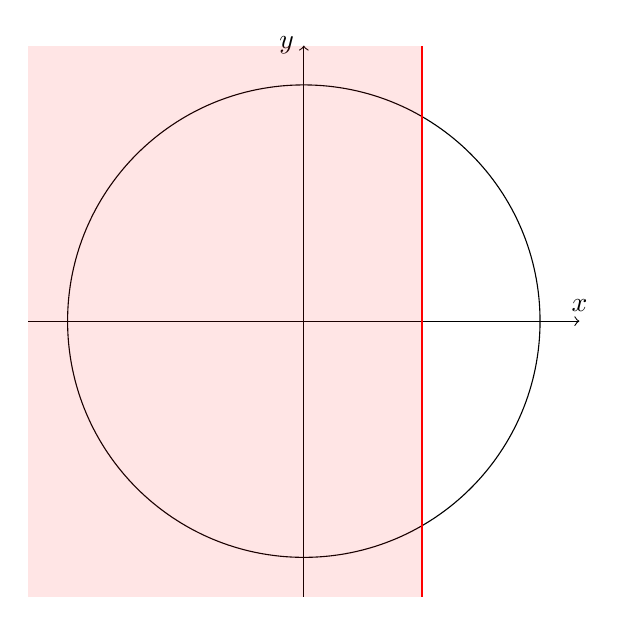
\begin{tikzpicture}
          %\draw[very thin,lightgray] (-3,-3) grid (3,3);
          \draw[->] (-3.5,0)--(3.5,0) node[above]{$x$};
          \draw[->] (0,-3.5)--(0,3.5) node[left]{$y$};
          \draw (0,0) circle (3);
          %\draw[thick,red] (-3,0) node[fill=red,inner
          %  sep=1.5pt,shape=circle]{} -- (3/2,0) node[fill=red,inner
          %  sep=1.5pt,shape=circle,label=180:$\frac{1}{2}$]{};
          \fill[red,very nearly transparent] (-3.5,-3.5)--(3/2,-3.5)--(3/2,3.5)--(-3.5,3.5)--cycle;
          \draw[red,thick] (3/2,-3.5)--(3/2,3.5);
        \end{tikzpicture}
        % EJD: shade entire block
        &
        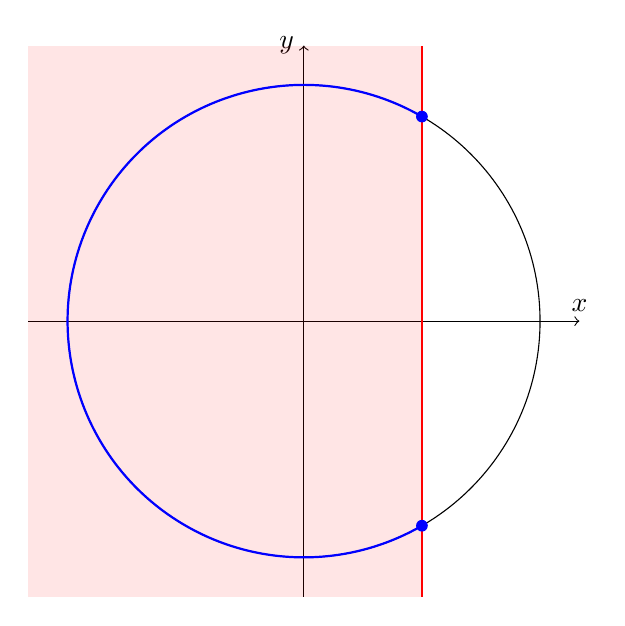
\begin{tikzpicture}
          %\draw[very thin,lightgray] (-3,-3) grid (3,3);
          \draw[->] (-3.5,0)--(3.5,0) node[above]{$x$};
          \draw[->] (0,-3.5)--(0,3.5) node[left]{$y$};
          \draw (0,0) circle (3);
          %\draw[thick,red] (-3,0) node[fill=red,inner
          %  sep=1.5pt,shape=circle]{} -- (3/2,0) node[fill=red,inner
          %  sep=1.5pt,shape=circle,label=270:$\frac{1}{2}$]{};
          \fill[red,very nearly transparent] (-3.5,-3.5)--(3/2,-3.5)--(3/2,3.5)--(-3.5,3.5)--cycle;
          \draw[red,thick] (3/2,-3.5)--(3/2,3.5);
          %\draw (0,0)--(60:3);
          %\draw (0,0)--(300:3);
          \draw[thick,blue] (60:3) node[fill=blue,inner
            sep=1.5pt,shape=circle]{} arc (60:300:3)
          node[fill=blue,inner sep=1.5pt,shape=circle]{};
        \end{tikzpicture}
        \\
        \mbox{(a) $\cos\theta\le 1/2\implies x\le 1/2$}
        &
        \mbox{(b) corresponding angles $\theta$}
        \end{array}$
      \caption{Solving the inequality $\cos\theta\le 1/2$ for $\theta$}
      \label{fig:costheta=1by2}
    \end{figure}
  \item %$\ds -2\sin x +1 \ge 0$ % EJD: better problem if original
        %ineq is \le , or involves -1/2, or is strict
    Solve for $\sin\theta$:
    \begin{equation*}
      -2\sin\theta + 1 \ge 0 
      \implies
      -2\sin\theta \ge -1
      \implies 
      \sin\theta \le \frac{1}{2}
    \end{equation*}
    Note the reversal of the inequality!

    Now, the condition $\sin\theta\le 1/2$ translates to $x\le 1/2$;
    see Figure~\ref{fig:-2sintheta+1GE0}(a).
    Then find all corresponding points on the circle, and the
    corresponding angles; see Figure~\ref{fig:-2sintheta+1GE0}(b).
    We see from the latter diagram and a couple of $1$, $2$,
    $\sqrt{3}$ triangles (not pictured) that the angles $\theta$ satisfying
    the inequality are given by $0\le\theta\le \pi/6$ or $5\pi/6\le
    \theta\le 2\pi$.
    \begin{figure}[htbp]
      \centering
      $\begin{array}{c@{\hspace{1cm}}c}
        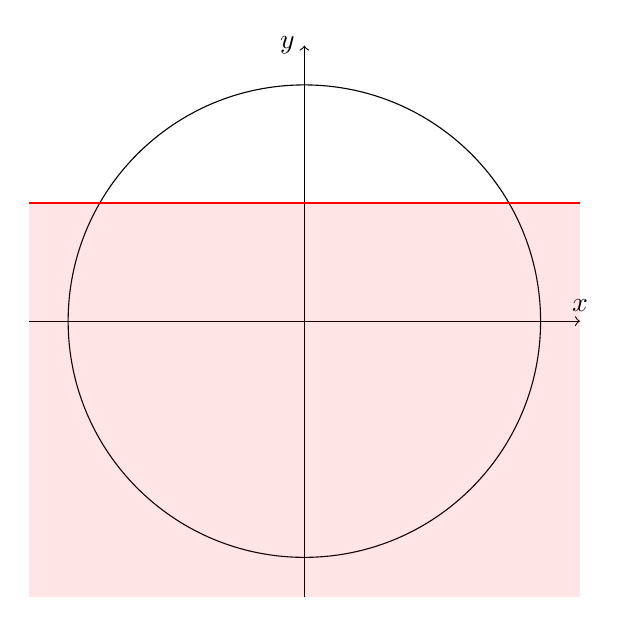
\begin{tikzpicture}
          %\draw[very thin,lightgray] (-3,-3) grid (3,3);
          \draw[->] (-3.5,0)--(3.5,0) node[above]{$x$};
          \draw[->] (0,-3.5)--(0,3.5) node[left]{$y$};
          \draw (0,0) circle (3);
          %\draw[thick,red] (0,-3) node[fill=red,inner
          %  sep=1.5pt,shape=circle]{} -- (0,3/2) node[fill=red,inner
          %  sep=1.5pt,shape=circle,label=180:$\frac{1}{2}$]{};
          \fill[red,very nearly transparent] (-3.5,-3.5)--(3.5,-3.5)--(3.5,3/2)--(-3.5,3/2)--cycle;
          \draw[red,thick] (-3.5,3/2)--(3.5,3/2);
        \end{tikzpicture}
        % EJD: shade entire half plane
        &
        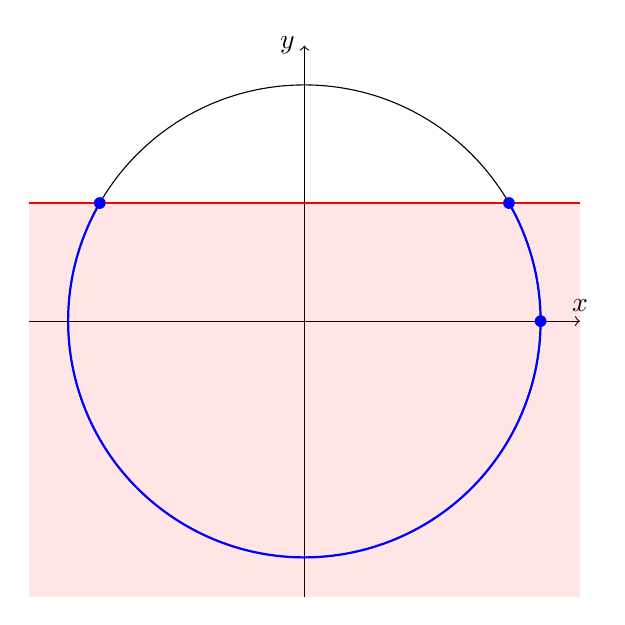
\begin{tikzpicture}
          %\draw[very thin,lightgray] (-3,-3) grid (3,3);
          \draw[->] (-3.5,0)--(3.5,0) node[above]{$x$};
          \draw[->] (0,-3.5)--(0,3.5) node[left]{$y$};
          \draw (0,0) circle (3);
          %\draw[thick,red] (0,-3) node[fill=red,inner
          %  sep=1.5pt,shape=circle]{} -- (0,3/2) node[fill=red,inner
          %  sep=1.5pt,shape=circle,label=180:$\frac{1}{2}$]{};
          \fill[red,very nearly transparent] (-3.5,-3.5)--(3.5,-3.5)--(3.5,3/2)--(-3.5,3/2)--cycle;
          \draw[red,thick] (-3.5,3/2)--(3.5,3/2);
          \draw[thick,blue] (150:3) node[fill=blue,inner
            sep=1.5pt,shape=circle]{} arc (150:360:3) arc (0:30:3)
          node[fill=blue,inner sep=1.5pt,shape=circle]{};
          \draw[blue] node[fill=blue,inner sep=1.5pt,shape=circle] (A)
          at (3,0) {};
        \end{tikzpicture}
        \\
        \mbox{(a) $\sin\theta\le 1/2\implies y\le 1/2$}
        &
        \mbox{(b) corresponding angles $\theta$}
        \end{array}$
      \caption{Solving the inequality $-2\sin\theta+1\ge 0$ for $\theta$}
      \label{fig:-2sintheta+1GE0}
    \end{figure}
  \item %$\ds -\frac{1}{\sqrt{3}} < \tan x < \sqrt{3}$
    In our framework, the inequality becomes
    \begin{equation*}
      -\frac{1}{\sqrt{3}} < \frac{y}{x} < \sqrt{3}
    \end{equation*}
    which can be interpreted as a condition on the slope of a line
    through the origin.  See
    Figure~\ref{fig:1osqrt3LTtanthetaLTsqrt3}(a). 
    Then find all corresponding points on the circle, and the
    corresponding angles; see Figure~\ref{fig:1osqrt3LTtanthetaLTsqrt3}(b).
    We see from the latter diagram and four $1$, $2$,
    $\sqrt{3}$ triangles (not pictured) that the angles $\theta$ satisfying
    the inequality are given by $0\le \theta <\pi/3$,
    $5\pi/6<\theta<4\pi/3$, or $11\pi/6<\theta\le 2\pi$.
    \begin{figure}[htbp]
      \centering
      $\begin{array}{c@{\hspace{1cm}}c}
        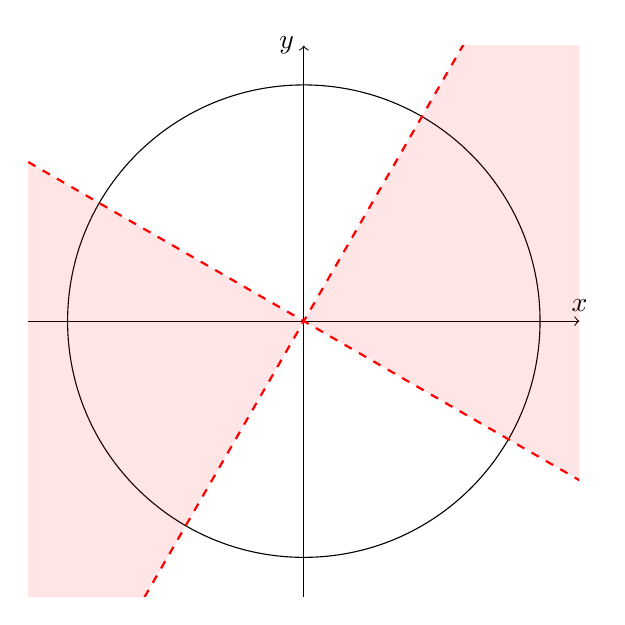
\begin{tikzpicture}
          %\draw[very thin,lightgray] (-3,-3) grid (3,3);
          \draw[->] (-3.5,0)--(3.5,0) node[above]{$x$};
          \draw[->] (0,-3.5)--(0,3.5) node[left]{$y$};
          \draw (0,0) circle (3);
          \clip (-3.5,-3.5) -- (3.5,-3.5) -- (3.5,3.5) -- (-3.5,3.5)
          -- cycle;
          \fill[red,very nearly transparent] (-3.5,{-3.5*sqrt(3)}) -- 
          (0,0) -- (-3.5,{-3.5/(-sqrt(3))}) -- cycle;
          \fill[red,very nearly transparent] (3.5,{3.5*sqrt(3)}) -- 
          (0,0) -- (3.5,{3.5/(-sqrt(3))}) -- cycle;
          \draw[red,thick,dashed]
          (-3.5,{-3.5*sqrt(3)})--(3.5,{3.5*sqrt(3)});
          \draw[red,thick,dashed]
          (-3.5,{-3.5/(-sqrt(3))}) -- (3.5,{3.5/(-sqrt(3))});
        \end{tikzpicture}
        &
        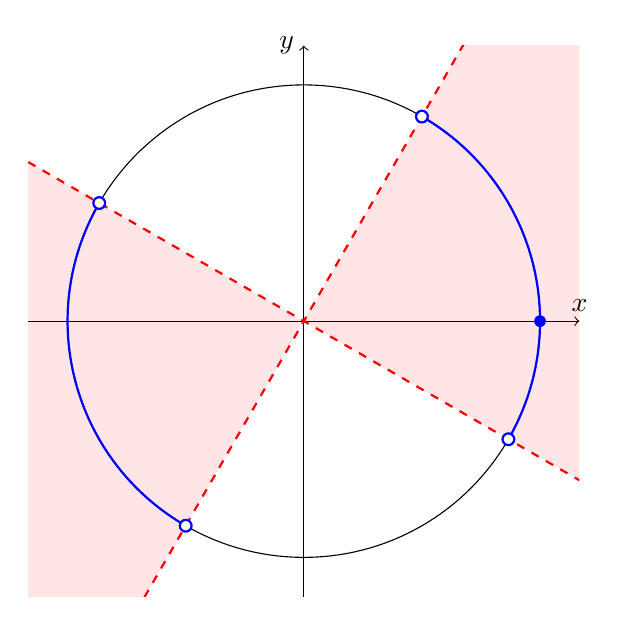
\begin{tikzpicture}
          %\draw[very thin,lightgray] (-3,-3) grid (3,3);
          \draw[->] (-3.5,0)--(3.5,0) node[above]{$x$};
          \draw[->] (0,-3.5)--(0,3.5) node[left]{$y$};
          \draw (0,0) circle (3);
          \clip (-3.5,-3.5) -- (3.5,-3.5) -- (3.5,3.5) -- (-3.5,3.5)
          -- cycle;
          \fill[red,very nearly transparent] (-3.5,{-3.5*sqrt(3)}) -- 
          (0,0) -- (-3.5,{-3.5/(-sqrt(3))}) -- cycle;
          \fill[red,very nearly transparent] (3.5,{3.5*sqrt(3)}) -- 
          (0,0) -- (3.5,{3.5/(-sqrt(3))}) -- cycle;
          \draw[red,thick,dashed] (-3.5,{-3.5*sqrt(3)})--(3.5,{3.5*sqrt(3)});
          \draw[red,thick,dashed]
          (-3.5,{-3.5/(-sqrt(3))}) -- (3.5,{3.5/(-sqrt(3))});
          \draw[thick,blue] (150:3) node[draw=blue,fill=white,inner
            sep=1.5pt,shape=circle]{} arc (150:240:3)
          node[draw=blue,fill=white,inner sep=1.5pt,shape=circle]{};
          \draw[thick,blue] (330:3) node[draw=blue,fill=white,inner
            sep=1.5pt,shape=circle]{} arc (330:360:3) arc (0:60:3)
          node[draw=blue,fill=white,inner sep=1.5pt,shape=circle]{};
          \draw[blue] node[fill=blue,inner sep=1.5pt,shape=circle] (A)
          at (3,0) {};
        \end{tikzpicture}
        \\
        \mbox{(a) $-1/\sqrt{3}<\tan\theta<\sqrt{3} 
          \implies -1/\sqrt{3}<y/x<\sqrt{3}$}
        &
        \mbox{(b) corresponding angles $\theta$}
        \end{array}$
      \caption{Solving the inequality $1/\sqrt{3}<\tan\theta<\sqrt{3}$ 
        for $\theta$}
      \label{fig:1osqrt3LTtanthetaLTsqrt3}
    \end{figure}
    % EJD: it would be nice if there were an inequality like a < y/x <
    % b to graph in Appendix B problems; could refer to it here.
  \item %$\ds \vphantom{\frac{1}{2}}\sin x < \cos x$
    The given condition becomes simply $y<x$, which is easy to graph;
    see Figure~\ref{fig:sinthetaLTcostheta}(a).
    Then find all corresponding points on the circle, and the
    corresponding angles; see Figure~\ref{fig:sinthetaLTcostheta}(b).
    We see from the latter diagram and a couple of $1$, $1$,
    $\sqrt{2}$ triangles (not pictured) that the angles $\theta$ satisfying
    the inequality are given by $0\le \theta < \pi/4$ or
    $5\pi/4<\theta <2\pi$.
    \begin{figure}[htbp]
      \centering
      $\begin{array}{c@{\hspace{1cm}}c}
        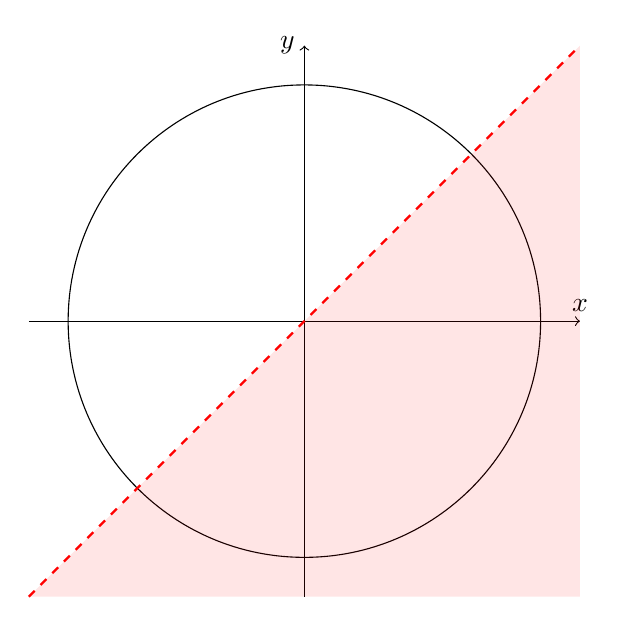
\begin{tikzpicture}
          %\draw[very thin,lightgray] (-3,-3) grid (3,3);
          \draw[->] (-3.5,0)--(3.5,0) node[above]{$x$};
          \draw[->] (0,-3.5)--(0,3.5) node[left]{$y$};
          \draw (0,0) circle (3);
          %\draw[thick,red] (0,-3) node[fill=red,inner
          %  sep=1.5pt,shape=circle]{} -- (0,3/2) node[fill=red,inner
          %  sep=1.5pt,shape=circle,label=180:$\frac{1}{2}$]{};
          \fill[red,very nearly transparent] (-3.5,-3.5)--(3.5,-3.5)--
          (3.5,3.5)--cycle;
          \draw[red,thick,dashed] (-3.5,-3.5)--(3.5,3.5);
        \end{tikzpicture}
        &
        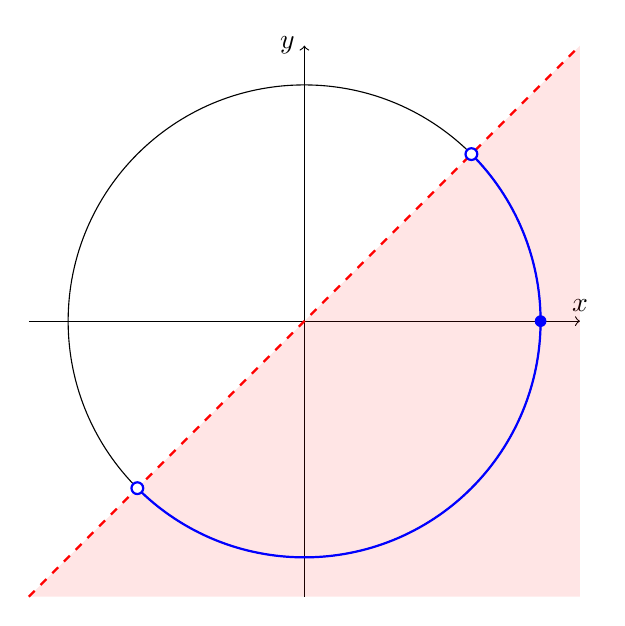
\begin{tikzpicture}
          %\draw[very thin,lightgray] (-3,-3) grid (3,3);
          \draw[->] (-3.5,0)--(3.5,0) node[above]{$x$};
          \draw[->] (0,-3.5)--(0,3.5) node[left]{$y$};
          \draw (0,0) circle (3);
          %\draw[thick,red] (0,-3) node[fill=red,inner
          %  sep=1.5pt,shape=circle]{} -- (0,3/2) node[fill=red,inner
          %  sep=1.5pt,shape=circle,label=180:$\frac{1}{2}$]{};
          \fill[red,very nearly transparent] (-3.5,-3.5)--(3.5,-3.5)--
          (3.5,3.5)--cycle;
          \draw[red,thick,dashed] (-3.5,-3.5)--(3.5,3.5);
          \draw[thick,blue] (225:3) node[draw=blue,fill=white,inner
            sep=1.5pt,shape=circle]{} arc (225:360:3) arc (0:45:3)
          node[draw=blue,fill=white,inner sep=1.5pt,shape=circle]{};
          \draw[blue] node[fill=blue,inner sep=1.5pt,shape=circle] (A)
          at (3,0) {};
        \end{tikzpicture}
        \\
        \mbox{(a) $\sin\theta<\cos\theta \implies y<x$}
        &
        \mbox{(b) corresponding angles $\theta$}
        \end{array}$
      \caption{Solving the inequality $\sin\theta<\cos\theta$ for $\theta$}
      \label{fig:sinthetaLTcostheta}
    \end{figure}
  \end{enumerate}
  % EJD: alternative: use graphs, see textbook solutions: 
  % ``my solutions are unusual but are
  % more compatible with the approach we have taken in this course so
  % far, so my solutions are hopefully easier for you to understand.''
% forward reference to 1.3
%\item (Based on D.77--82)
%  \begin{multicols}{4}
%  \begin{enumerate}
%  \item $\ds $
%  \item $\ds $
%  \item $\ds $
%  \item $\ds $
%  \end{enumerate}
%  \end{multicols}
\item %(Based on D.14) If a circle has radius 18 m, find the length of an arc
  %subtended by a central angle of $60^{\circ}$ degrees.
  We just use the formula for arc length $=r\theta$ where $\theta$ is
  the angle of the arc in radians.  We convert $60^{\circ}$ to
  radians: $60^{\circ} = 60^{\circ}\times 2\pi/360^{\circ} = \pi/3$,
  so the arc length is $r\theta = 18\pi/3 = 6\pi$ meters.
\item %(Based on D.15) A circle has radius 30 cm.  What angle is subtended at
  %the center of the circle by an arc 10 cm long?
  We have $10 = 30 \theta$ which implies $\theta=10/30 = 1/3$ radians
  or $1/3 \times 360/(2\pi) = 60/\pi \approx 19.1^{\circ}$.  
\item %(Based on D.42--58) Prove the following identities.
  \begin{enumerate}
  \item %$\ds \sin(2\pi - x) = -\sin x$
    By the angle subtraction formula, the LHS is
    \begin{equation*}
      \sin(2\pi - x) = \sin 2\pi \cos x - \cos 2\pi \sin x
      = 0 \cdot \cos x - 1 \sin x 
      = -\sin x
    \end{equation*}
    which is identical to the RHS.
  \item %$\ds (\sin x - \cos x)^2 = 1-\sin 2x$
    Squaring the RHS,
    \begin{equation*}
      \sin^2 x -2 \sin x \cos x + \cos^2 x 
      = \sin^2 x + \cos^2 x - 2\sin x \cos x
      = 1 - \sin 2x
    \end{equation*}
    by the Pythagorean identity and the double angle formula for $\sin$.
  \item %$\ds (\sin x + \sin y)(\sin x-\sin y) = \sin(x+y)\sin(x-y)$
    Expanding the LHS we have
    \begin{equation*}
      (\sin x +\sin y)(\sin x-\sin y) = \sin^2 x - \sin^2 y
    \end{equation*}
    Applying the product formula to the RHS,
    \begin{equation*}
      \sin(x+y)\sin(x-y) = \frac{1}{2}\left(
      \cos((x+y)-(x-y))-\cos((x+y)+(x-y))\right)
    \end{equation*}
    Simplifying, the RHS is
    \begin{equation*}
      \frac{1}{2}\left( \cos 2y - \cos 2x \right)
      = \frac{1}{2} \left( 1-2\sin^2 y - 1 + 2\sin^2 x \right)
      = \sin^2 x - \sin^2 y
    \end{equation*}
    which is identical with the LHS.
  \item %$\ds \sin 3\theta = 3\sin x - 4\sin^3 x $
    By the angle addition formula, the LHS is
    \begin{equation*}
      \sin 3\theta = \sin (\theta + 2\theta)
      = \sin\theta \cos 2\theta + \cos\theta \sin 2\theta
    \end{equation*}
    By the double angle formulas, the LHS is
    \begin{equation*}
      \sin\theta\cos 2\theta + \cos \theta\sin 2\theta
      = \sin\theta (1-2\sin^2\theta) + \cos\theta \cdot
      2\sin\theta\cos\theta
    \end{equation*}
    Simplifying and using $\cos^2\theta=1-\sin^2\theta$, the LHS is
    \begin{equation*}
      \sin\theta - 2\sin^3\theta + 2\cos^2\theta \sin \theta
      = \sin\theta -2\sin^3\theta + 2(1-\sin^2\theta)\sin\theta
      = 3\sin\theta - 4\sin^3\theta
    \end{equation*}
    which is identical to the RHS.
  \end{enumerate}
\item %(Based on D.59--64) If $\cos x=8/17$ and $\csc y = 2$, where $x$ and $y$
  %lie in the interval $[0,\pi/2]$, evaluate the following
  %expressions.
  Since $x$ and $y$ are in the first quadrant, we can use the
  reasoning of problem~\ref{prob:remaining} to determine
  \begin{equation*}
    \sin x = \frac{15}{17} \qquad \tan x = \frac{15}{8}
  \end{equation*}
  \begin{equation*}
    \sin y = \frac{1}{2} \qquad \cos y = \frac{\sqrt{3}}{2}
    \qquad \tan y = \frac{1}{\sqrt{3}}
  \end{equation*}
  \begin{enumerate}
  \item %$\ds \sin(x+y)$
    By the angle addition formula for $\sin$,
    \begin{equation*}
      \sin (x+y) = \sin x \cos y + \cos x \sin y
      = \frac{15}{17} \cdot \frac{\sqrt{3}}{2} + \frac{8}{17} \cdot
      \frac{1}{2}
      = \frac{15\sqrt{3}+8}{34}
    \end{equation*}
  \item %$\ds \cos(x-y)$
    By the angle subtraction formula for $\cos$,
    \begin{equation*}
      \cos(x-y) = \cos x \cos y + \sin x \sin y
      = \frac{8}{17} \frac{\sqrt{3}}{2} + \frac{15}{17} \frac{1}{2}
      = \frac{8\sqrt{3}+15}{34}
    \end{equation*}
  \item %$\ds \cos 2x$ % EJD: put this problem first in the list of four
    By the double angle formula for $\cos$,
    \begin{equation*}
      \cos 2x = 2\cos^2 x -1 = 2\left(\frac{8}{17}\right)^2 -1
      = -\frac{161}{289}
    \end{equation*}
  \item %$\ds \tan(x+y)$
    By the angle addition formula for $\tan$,
    \begin{equation*}
      \tan(x+y) = \frac{\tan x + \tan y}{1-\tan x \tan y}
      = \frac{15/8+ 1/\sqrt{3}}{1-(15/8)(1/\sqrt{3})}
      = \frac{15\sqrt{3}+8}{8\sqrt{3}-15}
    \end{equation*}
  \end{enumerate}
\item %(Based on D.39--41) Prove the following identities from the textbook.
  \begin{enumerate}
  \item %$\ds \vphantom{\frac{2}{2}}\sin 2x = 2\sin x \cos x$
    This is a consequence of the angle addition formula 
    \begin{equation*}
      \sin(x+y) = \sin x \cos y + \cos x \sin y
    \end{equation*}
    Letting $y=x$ we have
    \begin{equation*}
      \sin(x+x) = \sin x \cos x + \cos x \sin x
      \implies 
      \sin 2x = \sin x \cos x + \sin x \cos x = 2\sin x \cos x
    \end{equation*}
    as required.
  \item %$\ds \cos^2 x = \frac{1+\cos 2x}{2}$
    By the double angle formula for $\cos$, the RHS of the purported
    identity is
    \begin{equation*}
      \frac{1+\cos 2x}{2} = \frac{1+(2\cos^2 x -1)}{2}
      = \frac{2\cos^2 x}{2} = \cos^2 x
    \end{equation*}
    so is identical to the LHS.
  \end{enumerate}
\item %(Based on D.86) Use the subtraction formula for the sine function, namely
  %\begin{equation*}
  %  \sin(x-y) = \sin x \cos y - \cos x \sin y
  %\end{equation*}
  %to prove the addition formula for the sine function, namely
  %\begin{equation*}
  %  \sin(x+y) = \sin x \cos y + \cos x \sin y
  %\end{equation*}
  We just replace every $y$ in the subtraction formula with $-y$:
  \begin{equation*}
    \sin(x-y)=\sin x \cos y - \cos x \sin y
    \implies
    \sin(x-(-y)) = \sin x \cos (-y) - \cos x \sin(-y)
  \end{equation*}
  Now applying rules for even and odd functions,
  \begin{equation*}
    \sin (x+y) = \sin x \cos y - \cos x (-\sin y) = \sin x \cos y +
    \cos x \sin y
  \end{equation*}
  as required.
\end{enumerate}
\end{document}

